%
% Шаблон для ВКР бакалавра
%

\documentclass[a4paper,12pt]{article}
\usepackage[backend=biber,sorting=none,style=gost-numeric,autolang=other]{biblatex} % библиография
\usepackage{mathtext} %русские буквы в формулах
\usepackage[T2A]{fontenc}
\usepackage[utf8]{inputenc}
\usepackage[english,russian]{babel}
\usepackage{amsmath}
\usepackage{fancyvrb}
\usepackage{formular}
\usepackage{setspace} % управление междустрочными интервалами
%поля документа
\usepackage{tocloft}
\usepackage[left=3cm,right=1cm,top=2cm,bottom=2cm]{geometry}

\usepackage{misccorr} % точки в конце номеров разделов, использовать перед пакетом ccaption!
\usepackage{ccaption} % изменения подписей к рисункам и табл.

\usepackage[nooneline]{caption} 
\captionsetup[table]{justification=raggedright} % заголовок таблицы выравнивается влево
\captionsetup[figure]{justification=centering,labelsep=endash} % заголовок рисунка - по центру

% отступ перед первым абзацем
\usepackage{indentfirst}
%вставка изображений
\usepackage{graphicx}
% счетчики
\usepackage{totcount}
% управление содержанием
\usepackage{tocloft}
% управление таблицами и рисунками
\usepackage{float}

\usepackage{titlesec}

\newcounter{mycitecount}                                %% Счётчик библиографии
\AtEveryBibitem{\stepcounter{mycitecount}}              %% Работает для biblatex

\usepackage[figure,      %
            table,       %
            mycitecount, xspace ]{totalcount}           %% Подсчёт общего количества объектов в документе

% окружение для листингов - с нумерацией строк слева
\DefineVerbatimEnvironment{MyCode}{Verbatim}{frame=lines,numbers=left,numberblanklines=false,framesep=5mm}

% автоматическая нумерация листингов
\newfloat{Program}{phb}{lop}
\floatname{Program}{Листинг}
\floatstyle{ruled}

\captionsetup[Program]{justification=centering} % подпись к листингу - по центру

\setlength{\parindent}{1.25cm} % абзацный отступ в соответствии с ГОСТ

\setcounter{secnumdepth}{3} % глубина нумерации до подразделов

%если нужны точки в оглавлении для разделов - раскомментируйте следующую команду
%\renewcommand{\cftsecleader}{\cftdotfill{\cftdotsep}}

\addto\captionsrussian{%
\renewcommand{\figurename}{Рисунок}%
\renewcommand{\tablename}{Таблица}%
}

% дефис в подписи к рисункам
\captiondelim{ -- } 

% Настройки для окружений с подчеркиваниями для подписей и пр.
\setFRMfontencoding{T2A}
\setFRMdfontencoding{T2A}
% thanks to A.Starikov
\setFRMfontfamily{cmr}
\setFRMdfontfamily{ptm}
\setFRMdfontsize{10pt}

% задает длину поля для подписи на титульной странице
\newFRMfield{xtitlesign}{32mm}

% поле для факультета или кафедры
\newFRMfield{fcath}{65mm}

%имя файла с библиографией в формате BibTex
\addbibresource{rbiblio.bib}

% В соответствии с требованием: для списков использовать дефис
\renewcommand{\labelitemi}{--}
\titlespacing{\section}{\parindent}{12pt}{12pt}
\titlespacing{\subsection}{\parindent}{12pt}{12pt}
\titlespacing{\subsubsection}{\parindent}{12pt}{12pt}

\begin{document}

% счетчики страниц, рисунков, таблиц
\regtotcounter{page}
\regtotcounter{figure}
\regtotcounter{table}

\renewcommand{\refname}{\centerline{СПИСОК ИСПОЛЬЗОВАННЫХ ИСТОЧНИКОВ}} 
\renewcommand{\contentsname}{\centerline{СОДЕРЖАНИЕ}} 
%\renewcommand{\refname}{Список источников}  % По умолчанию "Список литературы" (article)
%\renewcommand{\bibname}{Литература}  % По умолчанию "Литература" (book и report)

% титульная страница
\thispagestyle{empty}
\begin{center} \small
\textbf{МИНИСТЕРСТВО НАУКИ И ВЫСШЕГО ОБРАЗОВАНИЯ\\ РОССИЙСКОЙ ФЕДЕРАЦИИ}\\
ФЕДЕРАЛЬНОЕ ГОСУДАРСТВЕННОЕ АВТОНОМНОЕ ОБРАЗОВАТЕЛЬНОЕ УЧРЕЖДЕНИЕ
ВЫСШЕГО  ОБРАЗОВАНИЯ\\
«Национальный исследовательский ядерный университет «МИФИ»\\
\textbf{Обнинский институт атомной энергетики} – \\
филиал федерального государственного автономного образовательного учреждения высшего\\
образования «Национальный исследовательский ядерный университет «МИФИ»\\
(ИАТЭ НИЯУ МИФИ)
\end{center}
%\vfill
\medskip

% Направление подготовки следует уточнять,
% магистры и бакалавры могут иметь разные наименования
\begin{center}
\begin{tabular}{rl}
Отделение & \useFRMfield{fcath}[\large Интеллектуальные кибернетические системы] \\ 
%Направление подготовки & \useFRMfield{fcath}[\large Информационные системы и технологии] \\ 
\end{tabular} 
\end{center}

\vfill

\large 

\begin{center}
\textbf{\Large Выпускная квалификационная работа --- } \\
\textbf{\Large бакалаврская работа}\\
	
	\medskip

{ \normalsize
по направлению подготовки  \textbf{09.03.02 Информационные  системы и технологии}\\

Направленность (профиль) \textbf{Информационные технологии}
}	
\vfill
\vfill
\medskip

\textbf{\Large 
		Разработка наземной системы позиционирования и навигации микродрона с применением компьютерного зрения
	}
	
\end{center}

\vspace{1cm}

\begin{tabular*}{\textwidth}{p{78mm}p{33mm}p{64mm}}
	Выполнил:\\студент гр. ИС-Б17 & \useFRMfield{xtitlesign} & Петренко В. Ю.\\
	& & \\
	Руководитель ВКР,\\к.т.н., доцент ОИКС & \useFRMfield{xtitlesign} & Мирзеабасов О. А. \\
	& & \\
	
	Нормоконтроль & \useFRMfield{xtitlesign} & Пичугина~И.А. \\
	& & \\
	% Если нужно добавить консультанта - раскомментируйте две строчки ниже
	Консультант ВКР бакалавра\\Инженер ЦОНД  & \useFRMfield{xtitlesign} & Турицын М. И.\\
	%& & \\
	Рецензент\\к.т.н., доцент ОЯФиТ   & \useFRMfield{xtitlesign} & Белоусов П. А.\\
	
	& & \\
	Выпускная квалификационная \\ работа допущена к защите & \useFRMfield{xtitlesign} &  \\
	& & \\
	Руководитель\\ образовательной программы \\
	09.03.02 Информационные системы и технологии\\
	канд. тех. наук  & \useFRMfield{xtitlesign} &Мирзеабасов~О.А. \\
	
\end{tabular*}


\vfill
\large

\begin{center}
Обнинск, 2021 г
\end{center}

\onehalfspacing

\pagebreak

% реферат
\thispagestyle{empty}

\section*{\centering РЕФЕРАТ}

\thispagestyle{empty} % страница реферата не нумеруется

Работа \total{page} стр., \total{table} табл., \total{figure} рис., \totalmycitecounts ист. 

БПЛА, КВАДРОКОПТЕР, РОБОТОТЕХНИКА, НАЗЕМНАЯ СТАНЦИЯ, КОМПЬЮТЕРНОЕ ЗРЕНИЕ, АВТОНОМНЫЙ ПОЛЕТ

Работа посвящена разработке экспериментального образца наземной станции и микродрона, а также выбору их протокола общения.
Суть работы заключается в модификации и доработке существующих робототехнических решений на основе БПЛА посредством выноса бортового компьютера в наземную станцию, благодаря чему станет возможно уменьшение размеров и стоимости квадрокоптера.
Наземная станция представляет собой совокупность компьютера и радиомодулей для получения и последующей обработки изображения с квадрокоптера. Результаты обработки отправляются по радио на борт квадрокоптера в виде управляющих сигналов.
Таким образом, квадрокоптер получает дополнительную систему координат без использования датчиков подобных GPS, а также возможность навигации с использованием компьютерного зрения.
% определяет свое место в пространстве 

Разработанный ПАК дает возможность создать образовательный робототехнический комплект на основе беспилотника. Вынося бортовой компьютер в наземную станцию, получаем такие преимущества, как безопасность, низкая стоимость, в том числе существенно удешевляется ремонт.

\pagebreak
\thispagestyle{empty}

\section*{\centering ОПРЕДЕЛЕНИЯ}

\thispagestyle{empty} % страница определений не нумеруется

Квадрокоптер --- БПЛА мультироторного типа с четырьмя несущими винтами

Бод-рейт -- скорость передачи данных через UART

Пропорционально-интегрально-дифференциальный регулятор (ПИД) – алгоритм автоматического управления, применяемый для стабилизации дрона

\pagebreak
\thispagestyle{empty}

\section*{\centering ОБОЗНАЧЕНИЯ И СОКРАЩЕНИЯ}

НИР --- Научно-исследовательская работа

БПЛА --- Беспилотный летательный аппарат

ПАК --- Программно-аппаратный комплекс

MAVLink -- Micro Air Vehicle Link

ROS -- Robotic Operating System

ВМГ -- Винто-моторная группа

FPV -- First Person View

OSD -- On Screen Display

UART -- Universal asynchronous receiver/transmitter

CSI -- Common System Interface

DSI -- Display Serial Interface

BEC -- Battery Eliminator Circuit

ESR -- Equivalent Series Resistance

AWG -- American Wire Gauge

ПИД регулятор -- Пропорционально-интегрально-дифференциальный регулятор

\pagebreak
\tocloftpagestyle{empty}
\tableofcontents

\thispagestyle{empty} % страница реферата не нумеруется
\pagebreak

\section*{\centering ВВЕДЕНИЕ}
\setcounter{page}{3}
\addcontentsline{toc}{section}{ВВЕДЕНИЕ}
Сфера беспилотных и робототехнических систем растет с неимоверной скоростью -- в 2020 году их количество увеличилось вдвое по сравнению с прошлым годом. На рынке труда спрос на специалистов данной области не удовлетворен и только растет. В связи с чем в программу основного общего образования включают курсы программирования и робототехники, становится популярной концепция STEM-образования, закупаются образовательные комплекты на основе квадрокоптеров \cite{minobr}.

Однако комплектов, способных удовлетворить спрос образовательных учреждений, не так много, самыми известными являются COEX Clover и Геоскан Пионер Мини.

Первый комплект представляет собой квадрокоптер диаметром до 300 мм с микрокомпьютером на борту, выполняющим все вычислительные операции. Даже штатное функционирование такого аппарата требует строгого соблюдения техники безопасности ввиду высокой травмоопасности, а внештатные ситуации приводят к серьезным поломкам с высокими затратами на ремонт. Из-за больших размеров возникает потребность в большом помещении, огражденном сеткой.

Набору Пионер Мини для автономных полетов внутри помещений требуются дополнительные датчики для его позиционирования, которые необходимо размещать в углах помещения. Эти устройства не входят в комплект и их стоимость превышает стоимость самого квадрокоптера. Помимо этого, проект с 2019 года не развивается.

В ходе эксплуатации комплекта COEX Clover в рамках участия в соревнованиях WorldSkills Russia <<Молодые профессионалы>> по направлению <<Эксплуатация беспилотных авиационных систем>> появилась идея, как усовершенствовать существующие комплекты.

Суть идеи заключается в выносе бортового компьютера квадрокоптера в наземную станцию, тем самым существенно уменьшая размер квадрокоптера. Такой квадрокоптер менее опасен, более устойчив к падениям и ударам и его стоимость получается ниже стоимости ближайших конкурентов. Наземная станция состоит из компьютера и совокупности программных модулей для получения и последующей обработки изображения с квадрокоптера. Результаты обработки являются координаты дрона. За счет wifi-соединения происходит отправка на борт дрона его координат и задание для автономной миссии. Таким образом, получается программно -- аппаратный комплекс из микродрона и наземной управляющей станции.

Цель настоящей работы разработать программно-аппаратный комплекс для создания образовательного робототехнического комплекта на базе БПЛА.
 % текст введения в файле intro.tex
\pagebreak
\pagebreak

\section{Глава 1. Обзор предметной области}

\subsection{Полетный контроллер}
\subsubsection{Семейства прошивок полетного контроллера}
Для получения данных с датчиков, обмена данными с периферией и управления моторной группой полетному контроллеру необходима прошивка.

Ввиду того, что нам может потребоваться доработка функционала прошивки полетного контроллера, мы не будем рассматривать прошивки с закрытым исходным кодом. Наряду с функционалом прошивки одним из ключевых факторов ее выбора будет тип открытой лицензии.

В семействе полетных контроллеров PixHawk наиболее популярны прошивки PX4 и Ardupilot. Эти прошивки активно используются как хоббистами, так и для решения профессиональных задач в промышленности и сфере эксплуатации БАС. Практически весь их функционал нацелен на выполнение автономных миссий. Ardupilot, в основном, разрабатывается и используется хоббийным сообществом. PX4 изначально был студенческой учебно-исследовательской работой, но сейчас его используют исследователи в области программирования, стабилизации и навигации БПЛА во всем мире.

Изначально это был студенческий НИР, но спустя 3 года вышел официальный релиз, сейчас его используют исследователи в области программирования, стабилизации и навигации БПЛА во всем мире. Главными особенностями PX4 являются поддержка огромного количества датчиков и навигация в режиме OFFBOARD, который позволяет управлять беспилотником при помощи бортового компьютера. OFFBOARD режим PX4 предоставляет огромные возможности для конфигурирования и управления полетным заданием с внешнего устройства, что подходит для поставленной задачи. Рассмотрим PX4 подробнее.

\subsubsection{PX4}
%\url{https://docs.px4.io/master/en/getting_started/px4_basic_concepts.html}
%\url{https://docs.px4.io/master/en/contribute/licenses.html}
%https://docs.px4.io/master/en/simulation/#simulator-mavlink-api

PX4 - прошивка с открытым исходным кодом, публикуемая под лицензией BSD-3-Clause. PX4 позволяет управлять различными типами беспилотников, включая: летательные (мультикоптеры, самолеты и вертолеты), наземные и подводные аппараты. Он совместим с большим количеством оборудования, датчиков и другой периферии. Позволяет реализовать гибкие режимы полета и функции безопасности.
Параметры PX4 настраиваются с помощью Q\-Ground\-Control \cite{px4}.

QGroundControl - кросплатформенный конфигуратор для настройки PX4 и Ardupilot прошивок. Он обеспечивает полное управление полетом и настройку беспилотника \cite{qgroundcontrol}.

PX4 для определения состояния аппарата, его стабилизации и автономного полета использует датчики, такие как: гироскоп, акселерометр, магнитометр (компас) и барометр. Для включения всех автоматических режимов и некоторых вспомогательных требуется GPS или другая система позиционирования.
Для передачи данных / телеметрии между наземной станцией управления, такой как Q\-Ground\-Control, и беспилотником, работающим под управлением PX4 может использоваться как проводное, так и беспроводное соединение по протоколу MAVLink. Он позволяет настраивать параметры во время полета, проверять телеметрию в режиме реального времени, менять миссию на лету и т. д.

PX4 можно управлять с отдельного компьютера через кабель или Wi-Fi. Дрон и компьютер обычно обмениваются данными с помощью API MAVLink, такого как MAVSDK или MAVROS \cite{px4}.

\subsubsection{MAVLink}

%\url{https://mavlink.io/en/}

MAVLink -- это протокол двоичной телеметрии, разработанный для систем с ограниченными ресурсами и каналов с ограниченной пропускной способностью. MAVLink был впервые выпущен в начале 2009 года Лоренцем Мейером (основателем PX4) и в настоящее время имеет значительное количество разработчиков. Протокол развернут в двух основных версиях: v1.0 и v2.0, которые имеют обратную совместимость (реализации v2.0 могут анализировать и отправлять пакеты v1.0).

MAVLink реализует гибрид шаблонов проектирования взаимодействия «публикация -- подписка» и «точка -- точка». В этом гибридном шаблоне потоки данных отправляются / публикуются как темы, а подпротоколы конфигурации, такие как протокол задания или протокол параметров, реализуются шаблоном «точка-точка» с повторной передачей.

Сообщения определяются в файлах XML. Каждый файл XML определяет набор сообщений, поддерживаемый MAVLink системой, также называемый «диалектом». Набор эталонных сообщений, который реализуется большинством наземных станций управления и автопилотов, определен в common.xml (большинство диалектов основано на этом определении).

Набор инструментов MAVLink использует определения XML сообщений для генерации библиотеки MAVLink для каждого из поддерживаемых языков программирования . Дроны, наземные станции управления и другие системы MAVLink используют сгенерированные библиотеки для связи. Они распространяются под лицензией MIT и поэтому могут использоваться без ограничений в любом приложении с закрытым исходным кодом без публикации исходного кода. MAVLink был впервые выпущен в начале 2009 года Лоренцем Мейером (основателем PX4) и в настоящее время имеет значительное количество разработчиков \cite{px}.

MAVLink поддерживает множество языков программирования, работающих на множестве микроконтроллеров / операционных систем (включая ARM7, ATMega, dsPic, STM32 и Windows, Linux, MacOS, Android и iOS). Допускает одновременно до 255 систем в сети (беспилотники, наземные станции и т. д.)

Обеспечивает как внешнюю, так и бортовую связь (например, между q\-ground\-con\-trol и дроном, а также между автопилотом дрона и камерой дрона с поддержкой MAVLink) \cite{mavlink}.

MAVLink развернут в двух основных версиях: v1.0 и v2.0, которые имеют обратную совместимость (реализации v2.0 могут анализировать и отправлять пакеты v1.0). Потоки телеметрических данных отправляются в многоадресном режиме, в то время как аспекты протокола, которые изменяют конфигурацию системы и требуют гарантированной доставки, являются point-to-point с повторной передачей.

%//переделать

Для того, чтобы запускать на наземной станции автономные миссии для БПЛА, необходим набор инструментов, позволяющий обрабатывать MAVLink сообщения, преобразовывать показания с камеры в координаты положения квадрокоптера и отправлять управляющие команды квадрокоптеру. Для выполнения обозначенного функционала можно использовать робототехнические фреймворки. Наиболее популярным робототехническим фреймворком является ROS.
% дописать про офборд
\subsection{Robotic Operating System}
%\url{https://www.ros.org/about-ros/}

Robotic Operating System (далее ROS) -- это гибкая платформа для написания программного обеспечения для роботов; набор инструментов, библиотек и соглашений, которые призваны упростить задачу создания сложного и надежного поведения роботов на самых разных роботизированных платформах \cite{ros}.

Целью создания ROS является создание среды разработки, которая позволяет разработчикам ПО для роботов взаимодействовать на глобальном уровне.

ROS сосредоточена на максимизации повторного использования кода при разработке. Основные характеристики, позволяющие это реализовать:

Распределенные процессы. Структура ROS создана в виде минимальных единиц исполняемых процессов (нод), и каждый процесс выполняется изолированно. Взаимодействие разных нод происходит только на уровне обмена сообщениями.

Управление пакетами. Несколько процессов, имеющих общую задачу, объединяются в пакеты. Управление пакетами подразумевает набор утилит, позволяющих автоматически скачивать, устанавливать и удалять пакеты. Пакетный менеджер гарантирует работоспособность и целостность установленных пакетов.

Публичные репозитории и документация. Каждый доступный пакет публикуется в публичном репозитории. Документация пакетов публикуется в единой системе, которая упрощает поиск необходимых пакетов.

Единое API. При разработке программы, использующей ROS, вы получаете простое и легко встраиваемое API. При этом при использовании API нет разницы, на каком языке была написана программа.

Поддержка различных языков программирования. ROS предоставляет клиентские библиотеки для поддержки различных языков программирования. Наиболее популярны Python, C ++, а также такие языки, как Lisp, JAVA, C\#, Lua и Ruby \cite{voltbro}.

Рассмотрим концепции ROS: ноды, топики, сервисы.

\subsubsection{Ноды}
Нода представляет собой процесс, который выполняет вычисления. Ноды объединяются в граф и взаимодействуют друг с другом с помощью топиков, сервисов и сервера параметров. Ноды предназначены для работы в мелкомасштабном масштабе; система управления роботом обычно состоит из множества нод.

Все ноды имеют имя ресурса графа, которое однозначно идентифицирует их для остальной системы. Ноды также имеют типы, который упрощает процесс обращения к исполняемому файлу узла в файловой системе. Эти типы представляют собой имена ресурсов пакета с именем пакета ноды и именем исполняемого файла ноды. Чтобы определить тип ноды, ROS ищет все исполняемые файлы в пакете с указанным именем и выбирает первый из найденных \cite{ros}. 
% http://wiki.ros.org/Nodes \cite{ros}

%ROS-нода – это специальная программа (обычно написанная на Python или C++), которая взаимодействует с другими нодами посредством ROS-топиков и ROS-сервисов. Разделение сложных робототехнических систем на изолированные ноды дает определенные преимущества: понижается связанность кода, повышается переиспользуемость и надежность.

Очень многие робототехнические библиотеки и драйвера выполнены в виде ROS-нод.
Для того, чтобы преобразовать обычную программу в ROS-ноду, необходимо подключить к ней библиотеку rospy или roscpp и добавить инициализирующий код.

Пример ROS-ноды на языке Python:

\begin{Program}[H]
	\caption{Пример ROS-ноды на языке Python} \label{lst:1}
	\begin{MyCode}
		import rospy
		
		rospy.init_node('my_ros_node')  # имя ROS-ноды
		
		rospy.spin()  # входим в бесконечный цикл...
	\end{MyCode}
\end{Program}

Возможность запуска нескольких нод в одном процессе осуществляет пакет nodelet. Он позволяет производить обмен сообщений внутри процесса без затрат на копирование \cite{ros}.
%http://wiki.ros.org/nodelet

\subsubsection{Топики}
Топиками называют шины, по которым ноды обмениваются сообщениями. Топики имеют семантику анонимной публикации/подписки, которая отделяет производство информации от ее потребления. Как правило, ноды не знают, с кем они общаются. Вместо этого ноды, которые заинтересованы в данных, подписываются на соответствующие топики; ноды, которые генерируют данные, публикуются в соответствующем топике. У топиков может быть несколько издателей и подписчиков.

Топики предназначены для однонаправленного потокового общения.

Каждый топик строго типизирован в соответствии с типом сообщения ROS, используемым для публикации в ней, и ноды могут получать сообщения только с совпадающим типом. Master не обеспечивает согласованность типа среди издателей, но абоненты не будут устанавливать сообщение транспорта, если топики не совпадают. Кроме того, все клиенты ROS проверяют совпадение MD5, вычисленного из файлов msg. Эта проверка гарантирует, что ноды ROS были скомпилированы из согласованных кодовых баз \cite{ros}.
% http://wiki.ros.org/Topics

\begin{Program}[H]
	\caption{Пример публикации сообщения типа std\_msgs/String (строка) в топик foo на языке Python} \label{lst:2}
	\begin{MyCode}
		from std_msgs.msg import String
		
		# создаем Publisher'а
		foo_pub = rospy.Publisher('/foo', String, queue_size=1)
		
		# публикуем сообщение
		foo_pub.publish(data='Hello, world!')
	\end{MyCode}
\end{Program}
\begin{Program}[H]
	\caption{Пример подписки на топик /foo на языке Python} \label{lst:3}
	\begin{MyCode}
		def foo_callback(msg):
		print msg.data
		
		#При получении сообщения в топик /foo
		#будет вызвана функция foo_callback.
		rospy.Subscriber('/foo', String, foo_callback)
	\end{MyCode}
\end{Program}

Также существует возможность работы с топиками с помощью утилиты rostopic. Например, с помощью следующей команды можно просматривать сообщения, публикуемые в топик /mavros/state:
\$ rostopic echo /mavros/state
\subsubsection{Сервисы}

Сервис -- это некоторый аналог функции, которая может быть вызвана из одной ноды, а обработана в другой. У сервиса есть имя, аналогичное имени топика, и 2 типа сообщений: тип запроса и тип ответа \cite{clover}.

\begin{Program}[H]
	\caption{Пример вызова ROS-сервиса из языка Python} \label{lst:4}
	\begin{MyCode}
		from clover.srv import GetTelemetry
		
		# Создаем обертку над сервисом get_telemetry
		# пакета clover с типом GetTelemetry:
		get_telemetry = rospy.ServiceProxy('get_telemetry',
						  srv.GetTelemetry)
		
		# Вызываем сервис и получаем телеметрию квадрокоптера:
		telemetry = get_telemetry()
		# С сервисами можно также работать при помощи утилиты rosservice.
		# Так можно вызвать сервис /get_telemetry из командной строки:
		
		rosservice call /get_telemetry "{frame_id: ''}"
	\end{MyCode}
\end{Program}

\subsubsection{MAVROS}
%\url{https://clover.coex.tech/ru/mavros.html}
%\url{https://dev.px4.io/master/en/ros/mavros\_installation.html}
Так как мы выбрали ROS как основной фреймворк для реализации нашего решения и MAVLink, в качестве основного протокола -- нам необходим компонент, обеспечивающий взаимодействие обозначенных систем.
MAVROS (MAVLink + ROS) -- это пакет для ROS, предоставляющий возможность управлять беспилотниками по протоколу MAVLink. MAVROS поддерживает полетные стеки PX4 и APM. Связь организовывается по UART, USB, TCP или UDP.

MAVROS подписывается на определенные ROS-топики в ожидании команд, публикует в другие топики телеметрию, и предоставляет сервисы.
Пакет mavros обеспечивает расширяемую связь MAVLink между компьютерами, на которых работает ROS, автопилоты с поддержкой MAVLink и GCS с поддержкой MAVLink. Нода MAVROS запускается в launch-файле \cite{clover}.

Прошивка рх4 позволяет использовать внешние системы видеонавигации, рассмотрим подробнее некоторые из них.
%MAVROS -- это «официальный» поддерживаемый мост между ROS и протоколом MAVLink. В настоящее время он расширяется, чтобы включить обмен сообщениями fast-RTPS, включая уровень для преобразования сообщений uORB PX4 в общие идиомы ROS. Эти расширения в последующем могут существенно улучшить скорость работы разрабатываемого решения.
%https://dev.px4.io/v1.9.0/en/setup/fast-rtps-installation.html доработать
\subsection{Потоковая передача видео}

\subsubsection{GStreamer}

GStreamer -- это библиотека для построения графиков компонентов обработки мультимедиа. Он поддерживается различными мультимедийными приложениями, позволяет осуществлять потоковую передачу аудио / видео и обрабатывать звук / видео. GStreamer является свободным программным обеспечением с лицензией GNU LGPL.

Практически все в GStreamer является элементом. Все, начиная от обычных источников потоков (filesrc, alsasrc, и т. п.), обработчиков потоков (демультиплексоры, декодеры, фильтры, и т. п.) и заканчивая конечными устройствами вывода (alsasink, fakesink, filesink, и т. п.).

Pad — это некая точка подключения одного элемента к другому, если более просто — это входы и выходы элемента (рис. \ref{fig:ris1}). Обычно они именуются «sink» — вход и «src» — выход.
% ~\ref{fig:ris1}
\begin{figure}[H]
	\centering
	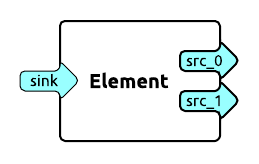
\includegraphics[width=0.5\linewidth]{pics/pic1}
	\caption{ GStreamer pads (sink, src\_0, src\_1)
	}
	\label{fig:ris1}
\end{figure}
Жизненный цикл элементы проводят внутри контейнеров. Контейнер управляет рассылкой сообщений от элемента к элементу, статусами элементов. Контейнеры делятся на два вида: Bin и Pipeline.

Bin -- простой контейнер, который управляет рассылкой сообщений от элемента к элементу которые находятся внутри него. Bin обычно используется для создания группы элементов которые должны совершать какое-либо действие. 
Pipeline является контейнером верхнего уровня, он управляет синхронизацией элементов, рассылает статусы. Например, если pipeline установить статус PAUSED, этот статус будет автоматически разослан всем элементам которые находятся внутри него. Pipeline является реализацией Bin \cite{gstreamer}. 

Источники данных -- это класс плагинов GStreamer, который позволяет читать медиаданные из различных источников, таких как файловая система или аудио-входы звуковой карты. Также, они позволяют получать медиапоток с различных серверов потокового вещания, таких как HTTP (ICECast, ShoutCast), RTSP, RTMP, TCP и UDP. 

Утилита gst-launch-1.0 позволяет запускать GStreamer pipeline без написания кода. Запуск pipeline имеет следующий вид:
gst-launch-1.0 описание-pipeline

Описание pipeline, в свою очередь, делится на описание элементов вида:
element1 property1=value1 property2=value2 ! element2.

Есть элемент типа element1 со свойствами property1 и property2, которые имеют значения value1 и value2 соответственно, и есть элемент типа element2. Символ «!» указывает на то, что выход element1 необходимо соединить с входом element2.
%https://habr.com/ru/post/179167/
% https://docs.gstreamer.com/documentation/
В случае с Raspberry источником видеопотока (element1) является rpicamsrc, который захватывает изображение с RPi камеры. rpicamsrc может выводить видео в виде необработанных кадров или закодированное в формате (M)JPEG или H.264 \cite{gstreamer1}. В качестве element2 будет выступать устройство вывода udpsink,-- это сетевой приемник, который отправляет UDP-пакеты в сеть.
%https://gstreamer.freedesktop.org/documentation/udp/udpsink.html
Для приема и обработки видеопотока на наземной станции может быть использован gscam.

\subsubsection{gscam}
gscam -- ROS драйвер, изначально разработанный для трансляции видеопотока на основе gstreamer через стандартный API камеры ROS. Его можно установить из стандартных репозиториев, предоставляемых менеджером apt или собрать вручную с помощью catkin\_make. gscam может быть запущен и как нода, и как нодлет.

gscam может подключаться к специально отформатированному конвейеру. При условии, что этот конвейер обрабатывает видео в формате RGB. gscam ожидает, что переменная окружения GSCAM\_CONFIG будет содержать gstreamer определение конвейера для его запуска.
gscam получает стрим и публикует 2 топика: /camera/image\_raw(необработанное изображение) и /camera/camera\_info(содержит калибровку камеры и дополнительные данные о конфигурации камеры) \cite{ros}.
% http://wiki.ros.org/gscam

\subsubsection{aruco\_gridboard}
Нода aruco\_gridboard подписывается на топики, публикуемые gscam: топик изображения /camera/image и топик /camera/camera\_info, содержащий параметры камеры. При получении видеопотока aruco\_gridboard распознает карту aruco маркеров, описанную в файле yaml, и публикует статус в топик /vision/status, а полученные координаты в /vision/pose.

Таким образом, видео с Raspberry Pi c помощью gstreamer передается по UDP на ip-адрес наземной станции; нода gscam получает UDP-пакеты и публикует изображение в топики /camera/image\_raw и /camera/camera\_info; aruco\_gridboard подписывается на топики с изображением и информацией о камере и публикует сообщения о положении дрона относительно карты маркеров в /mavros/vision\_pose/pose топик.

%http://www.uco.es/investiga/grupos/ava/sites/default/files/GarridoJurado2014.pdf
  % первая глава - в файле part1.tex
\pagebreak

\section{Разработка микродрона}
\subsection{Разработка архитектуры микродрона}
\subsection{Выбор ПО полетного контроллера}
Ввиду того, что может потребоваться доработка функционала ПО (прошивки) полетного контроллера, не будем рассматривать прошивки с закрытым исходным кодом. Наряду с функционалом прошивки одним из ключевых факторов ее выбора будет тип открытой лицензии. Если взять во внимание наиболее популярные открытые прошивки для полетных контроллеров, то можно выделить 2 семейства: потомки MultiWii и прошивки под полетные контроллеры семейства PixHawk.

MultiWii -- прошивка, изначально разработанная для получения и обработки данных с гироскопов и акселерометров игровой консоли Nintendo Wii. Позже, на основе частей из консоли Nintendo Wii (акселерометр + гироскоп) и контроллера atmega, был спроектирован полетный контроллер, на который была установлена уже коптерная прошивка MultiWii \cite{multiwii}. Со временем платформа atmega перестала удовлетворять аппаратным критериям, и MultiWii перерос в BaseFlight, базирующийся на чипах семейства STM32, а он в свою очередь в CleanFlight. Разработчики CleanFlight разошлись во мнениях касаемо функционала прошивки и сделали следующие ответвления:
\begin{itemize}
	\item BetaFlight;
	\item INav;
	\item EmuFlight.
\end{itemize}

BetaFlight нацелен на гоночные квадрокоптеры. Основными особенностями являются: минимальная фазовая задержка, точное следование управляющему сигналу (setpoint) и поддержка огромного количества полетных контроллеров (target).
Стоит пояснить фразу "минимальная фазовая задержка". При фильтрации показаний гироскопа происходит сдвиг по фазе между исходным и фильтрованным сигналами, что приводит к запозданию реакции ПИД регулятора, и как итог -- ПИД осцилляции. Фильтры в BetaFlight оптимизированы для уменьшения фазовой задержки.

INav сфокусирован на навигационных возможностях. Позволяет выполнять полеты по точкам, исходя из данных, полученных периферией. Поддерживает различные платформы, включая БПЛА мультироторного и самолетного типов, сухопутные и водные управляемые модели.

EmuFlight предназначен для акробатических и кинематографических полетов. Позволяет настроить квадрокоптер на плавный полет, содержит множество алгоритмов для фильтрации шумов.

Среди описанных прошивок только INav имеет функционал для автономных полетов, но инструменты внешнего управления имеют весьма скудный функционал, потому такой вариант не подходит для решения поставленной задачи.

В семействе полетных контроллеров PixHawk наиболее популярны прошивки PX4 и Ardupilot. Эти прошивки активно используются как хоббистами, так и для решения профессиональных задач в промышленности и сфере эксплуатации БАС. Практически весь их функционал нацелен на выполнение автономных миссий. Ardupilot, в основном, разрабатывается и используется хоббийным сообществом. PX4 изначально был студенческой учебно-исследовательской работой, но сейчас его используют исследователи в области программирования, стабилизации и навигации БПЛА во всем мире.

Главными особенностями PX4 являются поддержка огромного количества датчиков и навигация в режиме OFFBOARD, который позволяет управлять беспилотником при помощи бортового компьютера. OFFBOARD режим PX4 предоставляет огромные возможности для конфигурирования и управления полетным заданием с внешнего устройства, что подходит для поставленной задачи. Рассмотрим PX4 подробнее.

%\url{https://docs.px4.io/master/en/getting_started/px4_basic_concepts.html}
%\url{https://docs.px4.io/master/en/contribute/licenses.html}
%https://docs.px4.io/master/en/simulation/#simulator-mavlink-api

PX4 -- прошивка с открытым исходным кодом, публикуемая под лицензией BSD-3-Clause. PX4 позволяет управлять различными типами беспилотников, включая: летательные (мультикоптеры, самолеты и вертолеты), наземные и подводные аппараты. Он совместим с большим количеством оборудования, датчиков и другой периферии. Позволяет реализовать гибкие режимы полета и функции безопасности.
Параметры PX4 настраиваются с помощью Q\-Ground\-Control \cite{px4}.

QGroundControl -- кросплатформенный конфигуратор для настройки PX4 и Ardupilot прошивок. Он обеспечивает полное управление полетом и настройку беспилотника \cite{qgroundcontrol}.

PX4 для определения состояния аппарата, его стабилизации и автономного полета использует датчики, такие как: гироскоп, акселерометр, магнитометр (компас) и барометр. Для включения всех автоматических режимов и некоторых вспомогательных требуется GPS или другая система позиционирования.
Для передачи данных / телеметрии между наземной станцией управления, такой как Q\-Ground\-Control, и беспилотником, работающим под управлением PX4 может использоваться как проводное, так и беспроводное соединение по протоколу MAVLink. Он позволяет настраивать параметры во время полета, проверять телеметрию в режиме реального времени, менять миссию на лету и т. д.

PX4 можно управлять с внешнего бортового компьютера или наземной станции через кабель или по радио каналу связи. Дрон и компьютер обычно обмениваются данными с помощью API MAVLink, такого как MAVSDK или MAVROS \cite{px4}.

\subsection{Компоненты квадрокоптера}

Набор наземной станции и квадрокоптера в основном планируется использовать в помещении в образовательных целях. При весе свыше 250 г требуется регистрация, согласно воздушному кодексу Российской Федерации \cite{ivp}. На основе эксплуатационных требований были поставлены следующие условия к собираемому квадрокоптеру:
\begin{itemize}
	\item размер не должен превышать 140*140*50 \(мм^3\);
	\item полетный вес должен быть ниже 250 г;
	\item пропеллеры должны быть защищены;
	\item низкая стоимость;
	\item ремонтопригодность;
	\item возможность выполнения автономной миссии;
	\item поддержка PX4;
	\item минимальное полетное время 5 мин;
	\item радиус действия сигнала не менее 50 м.
	% дописано
\end{itemize}

В ходе проведения анализа рынка радиоуправляемых квадрокоптеров было выявлено, что готовых вариантов, соответствующих вышеперечисленным условиям, нет. В связи с чем необходимо подобрать компоненты и собрать вручную.

Подходя к вопросу выбора рамы, стоит учитывать такие факторы как:
\begin{itemize}
	\item прочность рамы;
	\item легкий вес;
	\item диагональную жесткость;
	\item стоимость;
	\item монтажные отверстия на раме, совпадающие с отверстиями на электронике.
\end{itemize}

Диагональная жесткость важна для увеличения собственной частоты колебаний рамы. Чем больше собственная частота колебаний, тем меньше фильтрации требуется.

Фильтрация необходима, чтобы в алгоритм стабилизации приходил только полезный сигнал, очищенный от паразитных шумов.
Полезный сигнал представляет собой реальные физические движения дрона. В спектре данных гироскопа он находится в области низких частот, в то время как в верхних частотах находятся физические вибрации, вносимые компонентами дрона, а также вибрации, создаваемые электрическими помехами в цепи питания гироскопа.
При этом нужно учитывать, что помимо нефильтруемого диапазона низких частот (0 -- 20 / 80 Гц) в котором находятся реальные движения дрона, существует эффект фазового сдвига сигнала гироскопа при фильтрации, который увеличивается при уменьшении частоты среза фильтра. Таким образом, излишняя фильтрация приводит к ПИД осцилляциям и невозможности процесса регулирования.

Были проведены испытания с рамами из разных материалов. Рассматривались следующие альтернативы: фанера, PLA, PETG и угольно-армиро\-ван\-ный пластики, текстолит и углепластик (композитный пластик, также известный как карбон). Фанера обладает низкой стоимостью, но уступает по жесткости остальным альтернативам. PLA пластик самый безопасный для здоровья человека, им можно печатать детали на 3D принтере, но при этом обладает низкой устойчивостью к ударам. PETG обладает большей прочностью по сравнению с PLA, но недостаточно жесткий, в связи с чем уменьшается собственная частота колебаний рамы, изготовленной из данного материала. Угольно-армированный пластик позволяет обеспечить жесткость и прочность рамы, но является одним из самых дорогих вариантов и сопровождается трудностями печати.
Стеклотекстолит является самым жестким среди вышеперечисленных альтернатив, но обладает самым большим весом. Карбоновый композит самый дорогой из перечисленных, однако является самым прочным, жестким и относительно легким вариантом. Также в продаже имеется большое количество готовых рам из этого материала, которые могут удовлетворять поставленные условия, и если получится найти подходящий вариант, изготовление прототипа дрона обойдется выгоднее, чем при производстве рам поштучно. Таким образом, было решено использовать карбоновую раму.

В качестве защиты для пропеллеров выбран пластик, так как обладает упругостью и низкой стоимостью, имеются в продаже готовые варианты, а также возможна их печать на принтере.

Форм фактор рамы также является немаловажной деталью. Для выполнения задач позиционирования и навигации в зависимости от условий необходимо будет поворачивать камеру вниз, вперед и вверх. Исходя из этого, необходимо, чтобы защита пропеллеров, пластины рамы, а также аккумулятор не перекрывали обзор / уменьшали область видимости. Оптимальным решением является рама с вытянутым корпусом и расположением лучей по типу deadcat -- передние лучи разведены на угол, близкий к 180 градусам. Расстояние между отверстиями для монтажа электроники выгоднее выбирать из стандартов -- 16*16, 20*20 или 25,5*25,5 мм. Вариант 25,5*25,5 мм рассматривать стоит только в том случае, если необходимо использовать <<все в одном>>: плату, совмещающую полетный контроллер и регуляторы в одном устройстве. Для поставленной цели -- создания учебного набора квадрокоптера такая плата неуместна по следующим причинам:
\begin{itemize}
	\item в случае поломки заменяется полностью;
	\item стоимость выше, чем у комплекта раздельных регуляторов и полетного контроллера;
	\item выбор такого формата плат, с ресурсами, необходимыми для реализации проекта, крайне мал.
\end{itemize}

Основываясь на вышеперечисленном была приобретена рама, представленная на рисунке \ref{fig:frame}. Она позволяет установить нано камеру (размером 14*14 мм), стеки из полетного контроллера и регуляторов с посадочными отверстиями 20*20 мм / 16*16 мм, моторы размера 1102-1308 и пропеллеры диаметром до 40 мм (2.3").

\begin{figure}[H]
	\centering
	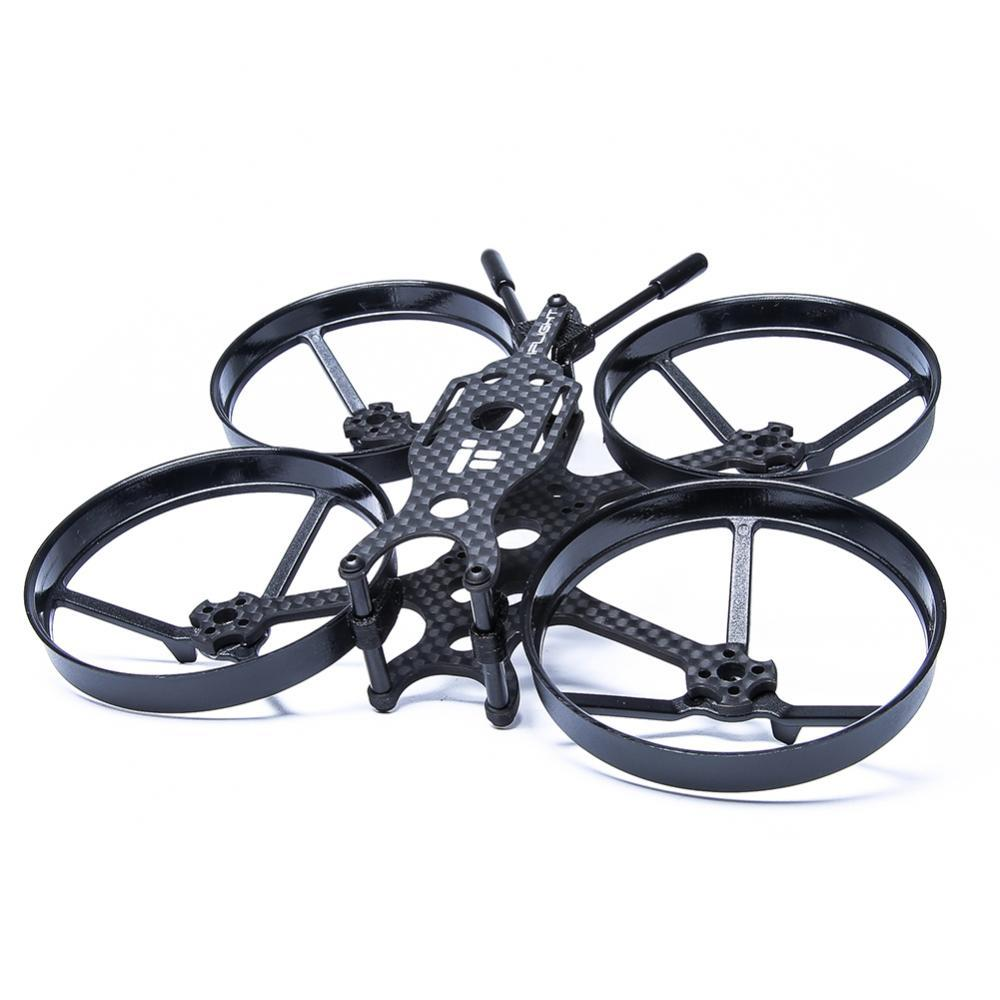
\includegraphics[width=0.5\linewidth]{../RW/pics/frame}
	\caption{Рама для экспериментального образца квадрокоптера
	}
	\label{fig:frame}
\end{figure}

Данная рама используется для создания экспериментального образца. В случае массового производства комплектов, которые будут получены при достижении поставленной цели, рама может быть заменена собственной разработкой.

Перейдем к выбору электроники.

Электроника квадрокоптера должна быть совместимой по характеристикам и габаритам. 

Для управления с наземной станции полетный контроллер должен:
\begin{itemize}
	\item обладать минимум 2 UART портами;
	\item быть совместимым с прошивкой PX4.
\end{itemize}

UART (Universal asynchronous receiver / transmitter) -- это аппаратный последовательный интерфейс, который позволяет подключать датчики и периферию к полетному контроллеру. У него есть два вывода для внешнего соединения: TX -- для передачи данных, RX -- для приема.

UART порты потребуются для подключения устройства приема -- передачи телеметрии и возможности подключения дополнительной периферии.

Выбор чипа процессора основан на требованиях к ресурсам по памяти, производительности и периферии. Для того, чтобы прошить PX4, необходим объем памяти процессора не ниже 1 МБ. Такое условие выполняют процессоры на базе F405 / F745 / F765 / H743. Сравнение характеристик процессоров представлены в таблице \ref{tab:tab1}. Преимущество F7 и H7 чипов в том, что обладают большими вычислительными способностями и ресурсами, но они дороже, выбор полетных контроллеров на таких чипах меньше, а разработка собственного полетного контроллера пока не целесообразна.


\begin{table}[h]
	\caption{Сравнение высокопроизводительных микроконтроллеров STM32} \label{tab:tab1}
	\centering
	\begin{tabular}{ | c | c | c | c |}
		\hline
		Название серии & F4 \cite{stm32f4} & F7 \cite{stm32f7} & H7 \cite{stm32h7}    \\ \hline
		Ядро & Cortex-M4F & Cortex-M7F  & Cortex-M7F   \\ \hline
		Макс. частота ядра & 180 & 216  & 480   \\ \hline
		Объем Flash памяти & 64-2056 & 64-2056  & 128 — 2048   \\ \hline
		Объем RAM памяти  & до 384 & 256-512  & до 1,4 МБайт   \\ \hline
		Особенности & до 4 UART & до 6 UART  & до 7 UART   \\
		\hline
	\end{tabular}
	\label{table:satellites}
\end{table}

Винто-моторная группа должна быть оптимизирована под задачи автономного полета в помещении на небольшой скорости. Под такую задачу подходит низкооборотистая ВМГ с максимально большим диаметром пропеллера и минимально возможным шагом, что дает небольшую скорость полета и максимальную статическую тягу. Под выбранную раму походят пропеллеры диаметром 2-2.3". Проведен анализ рынка и выбраны пропеллеры с диаметром 2.3" и шагом 3.5". При одинаковых объемах статора мотора крутящий момент на низких оборотах будет больше у того мотора, где больше диаметр статора, а на высоких оборотах там, где больше высота. Для экспериментального образца оптимальным выбором являются моторы 1202. В четырехзначном числе маркировки мотора первые две цифры отвечают за диаметр статора, вторые -- за высоту. Количество оборотов на вольт (kv) выбирается, учитывая напряжение аккумулятора. Чем больше напряжение, тем меньше количество оборотов на вольт должно быть на моторе. Каждая ячейка, подключенная последовательно увеличивает напряжение на 4.2 В в заряженном состоянии. Для квадрокоптера с диагональю рамы 120 мм по соотношению вес / токоотдача наиболее выгодно ставить аккумуляторы с 2-3 ячейками. Основываясь на таблице характеристик, приведенных производителем, были выбраны моторы с 6000 kv (рисунок \ref{fig:motor}).
Учитывая потребление тока моторами на полном газу и добавляя 10 -- 15 \% запаса, получаем характеристику регуляторов -- максимальный ток, проходящий через них. На экспериментальном образце он равен 15 А.
\begin{figure}[H]
	\centering
	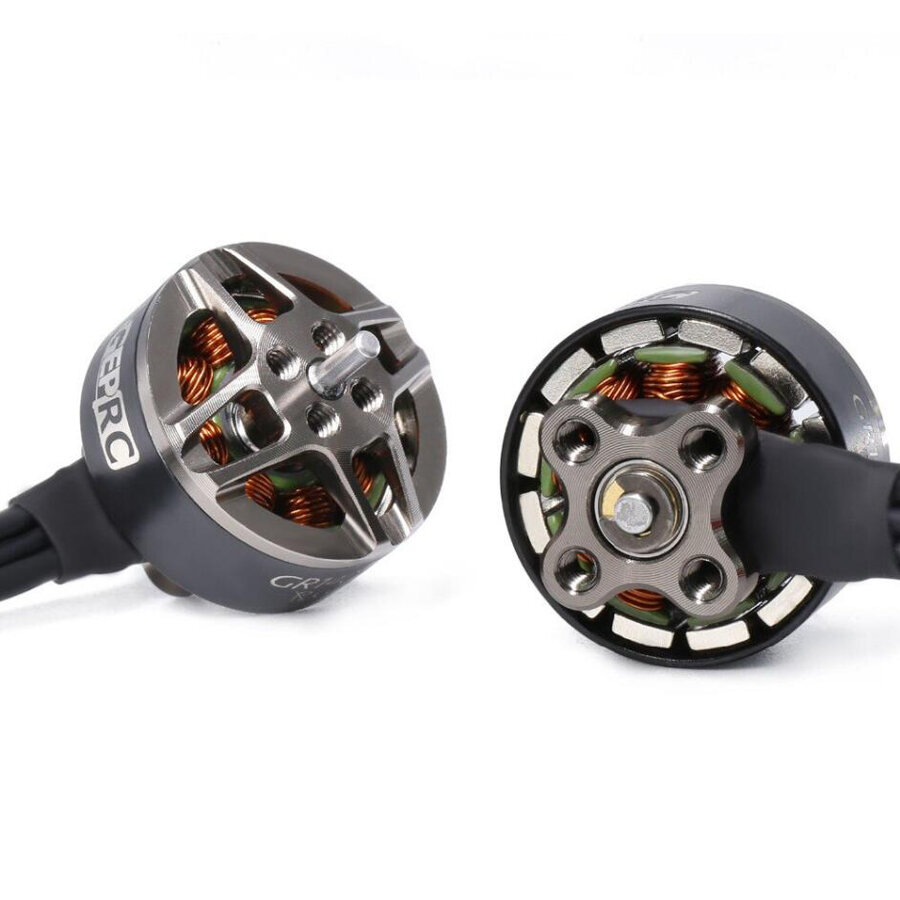
\includegraphics[width=0.5\linewidth]{../RW/pics/motor}
	\caption{Моторы для экспериментального образца квадрокоптера
	}
	\label{fig:motor} % эта метка позволяет ссылаться на рисунок в тексте
\end{figure}

\begin{figure}[H]
	\centering
	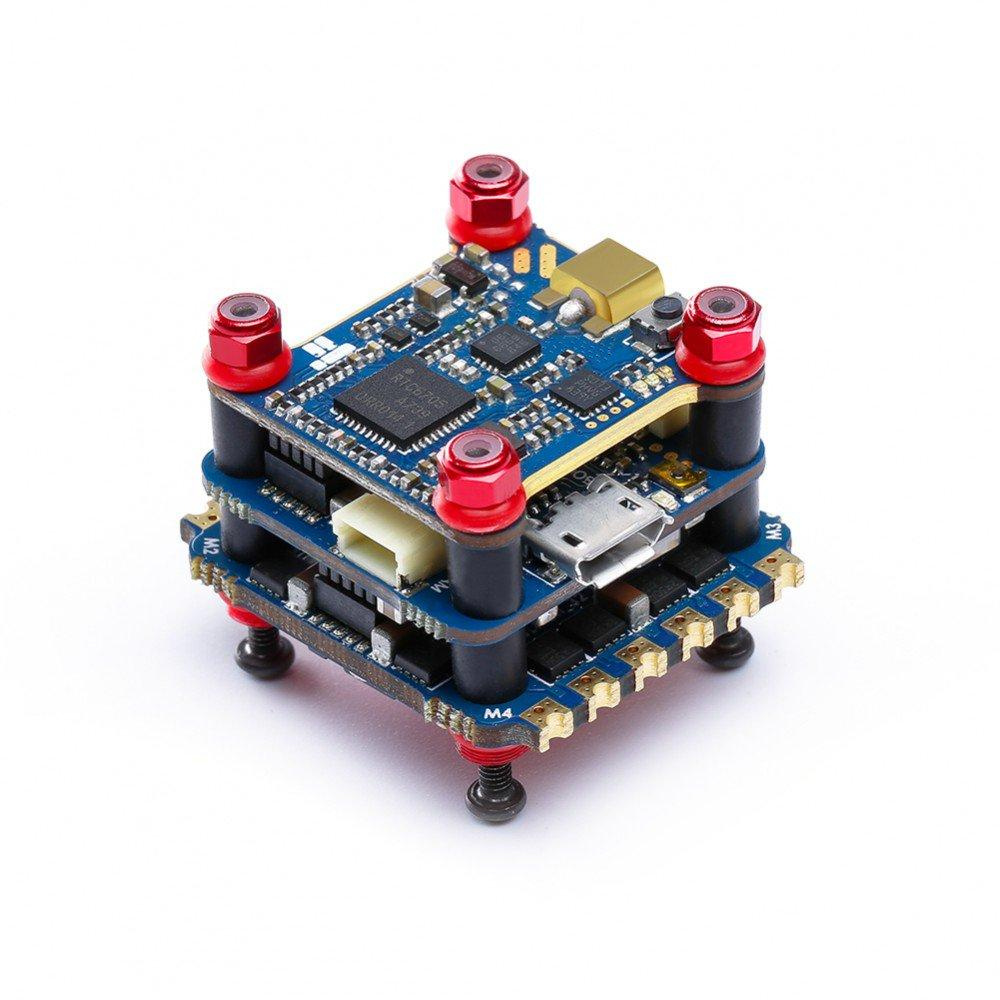
\includegraphics[width=0.5\linewidth]{../RW/pics/stack}
	\caption{Стек электроники для экспериментального образца квадрокоптера
	}
	\label{fig:stack} % эта метка позволяет ссылаться на рисунок в тексте
\end{figure}

Видеопередатчик и камера выбирались исходя из поставленных условий. Видеосигнал аналогового типа дешевле и передается с задержкой меньше, чем цифровой сигнал. MVP решение основывается на аналоговом сигнале. Так как необходимо будет передавать видеопоток, камера должна иметь максимально возможное количество телевизионных линий -- разрешающая способность (TVL). Для камер нано формата это 1000 TVL. Размер изображения может быть 4:3 и 16:9. Формат PAL / NTSC также может быть выбран на усмотрение.

Видеопередатчик обладает такими характеристиками как:
\begin{itemize}
	\item выходная мощность;
	\item выходная частота;
	\item количество каналов.
\end{itemize}

Для помещений нет необходимости использования высокой мощности видеопередачи, потому используется минимально возможная -- 25mW. Частота видеосигнала 5.8 ГГц.

Для общения с наземной станцией квадрокоптеру понадобятся устройства приема-передачи телеметрии. Протокол, бод-рейт (скорость передачи данных для подключенного устройства приема-передачи данных) и частота устройств станции и квадрокоптера должны совпадать. Для экспериментального образца были выбраны радиомодуль и приемник с поддержкой двусторонней телеметрии MAVLink на частоте 2.4 ГГц.

Из указанных компонентов был собран дрон (рисунок \ref{fig:drone}), подробный результат представлен в отчете научно-исследовательской работы \cite{nir1}. В ходе тестирования была выявлена высокая задержка (217 мс) при получении видеосигнала. Такая задержка обусловлена суммой задержек каждого устройства (камеры, видеопередатчика, видеоприемника, USB порта компьютера). Учитывая, что она также присутствует на устройстве приема-передачи телеметрии, затрудняется выполнение автономной миссии, поскольку от результата обработки видеопотока зависит реакция дрона. Результат не совпал с ожиданием, было необходимо провести исследование с использованием цифровой видеопередачи и сравнить результаты. В качестве видеопередатчика было решено использовать микрокомпьютер RPi, а запускать трансляцию видеопотока с помощью удаленного подключения по протоколу ssh.

\begin{figure}[H]
	\centering
	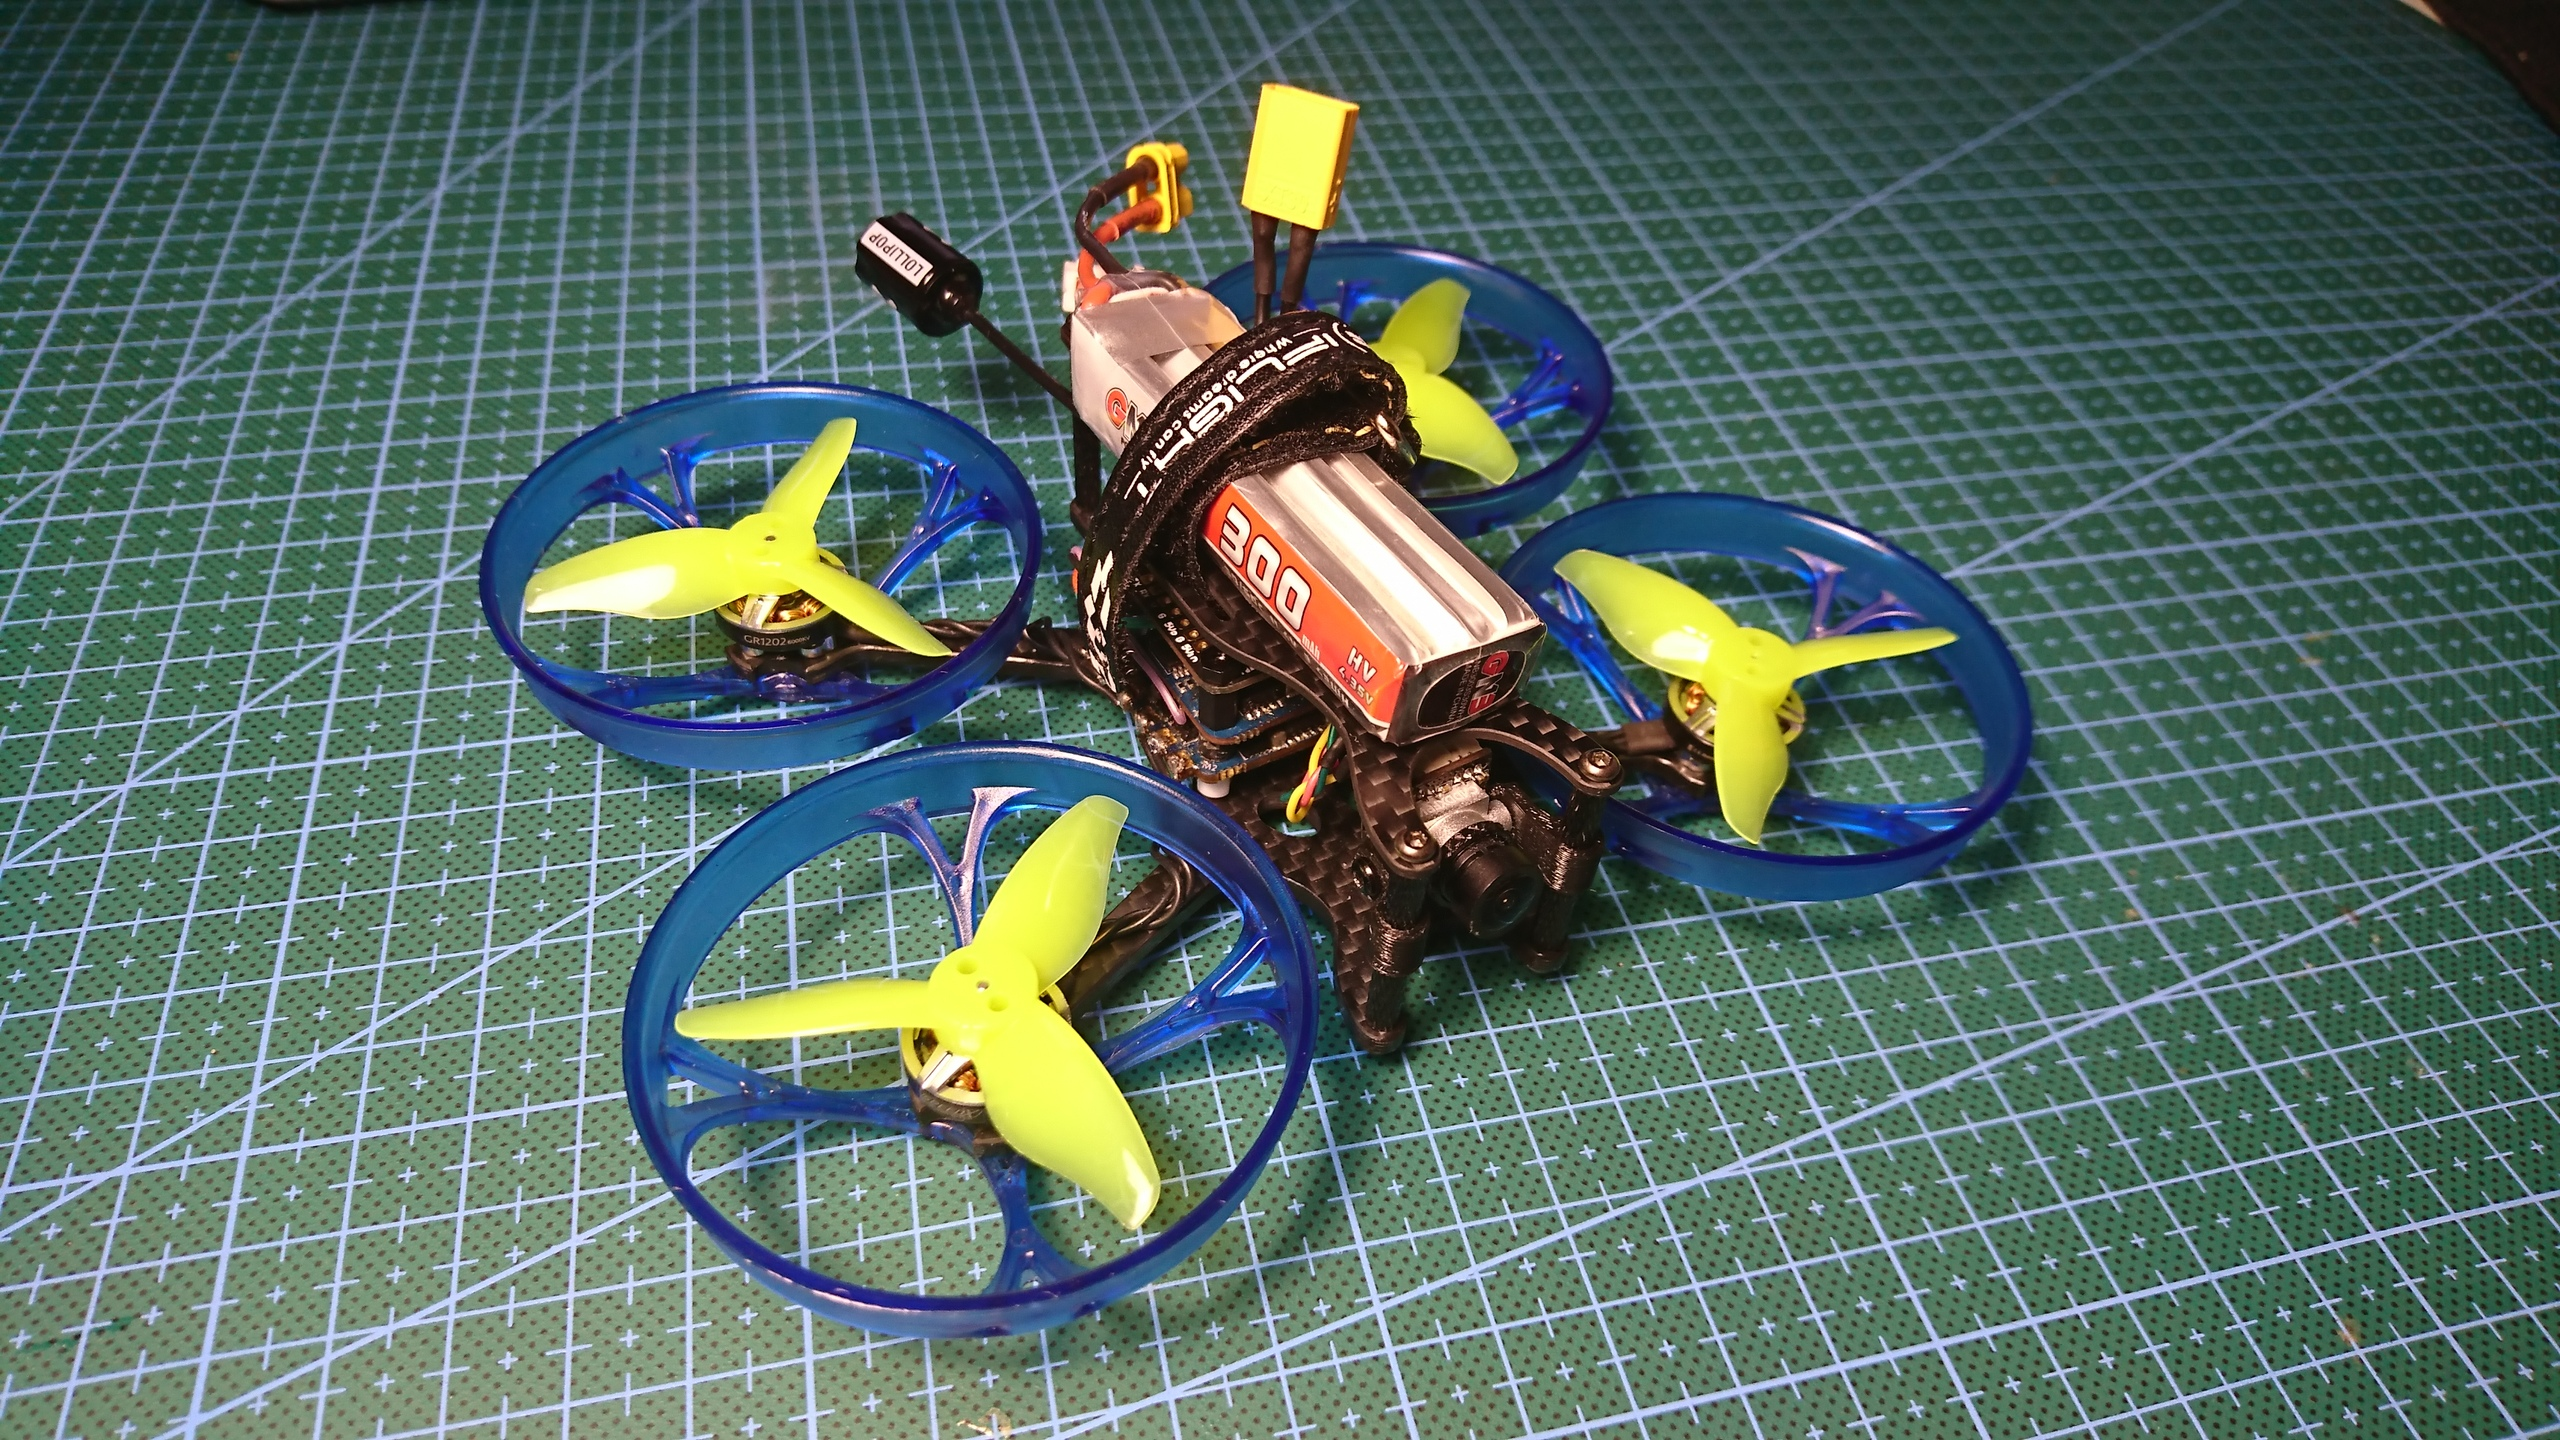
\includegraphics[width=0.5\linewidth]{../RW/pics/quad2}
	\caption{Первый экспериментальный образец дрона
	}
	\label{fig:drone} % эта метка позволяет ссылаться на рисунок в тексте
\end{figure}

В отчете научно-исследовательской работы \cite{nir2} представлен результат: задержка уменьшилась с 217 мс до 150 мс, а качество изображения значительно улучшилось (рисунки \ref{fig:time}, \ref{fig:zadergka}).

\begin{figure}[H]
	\centering
	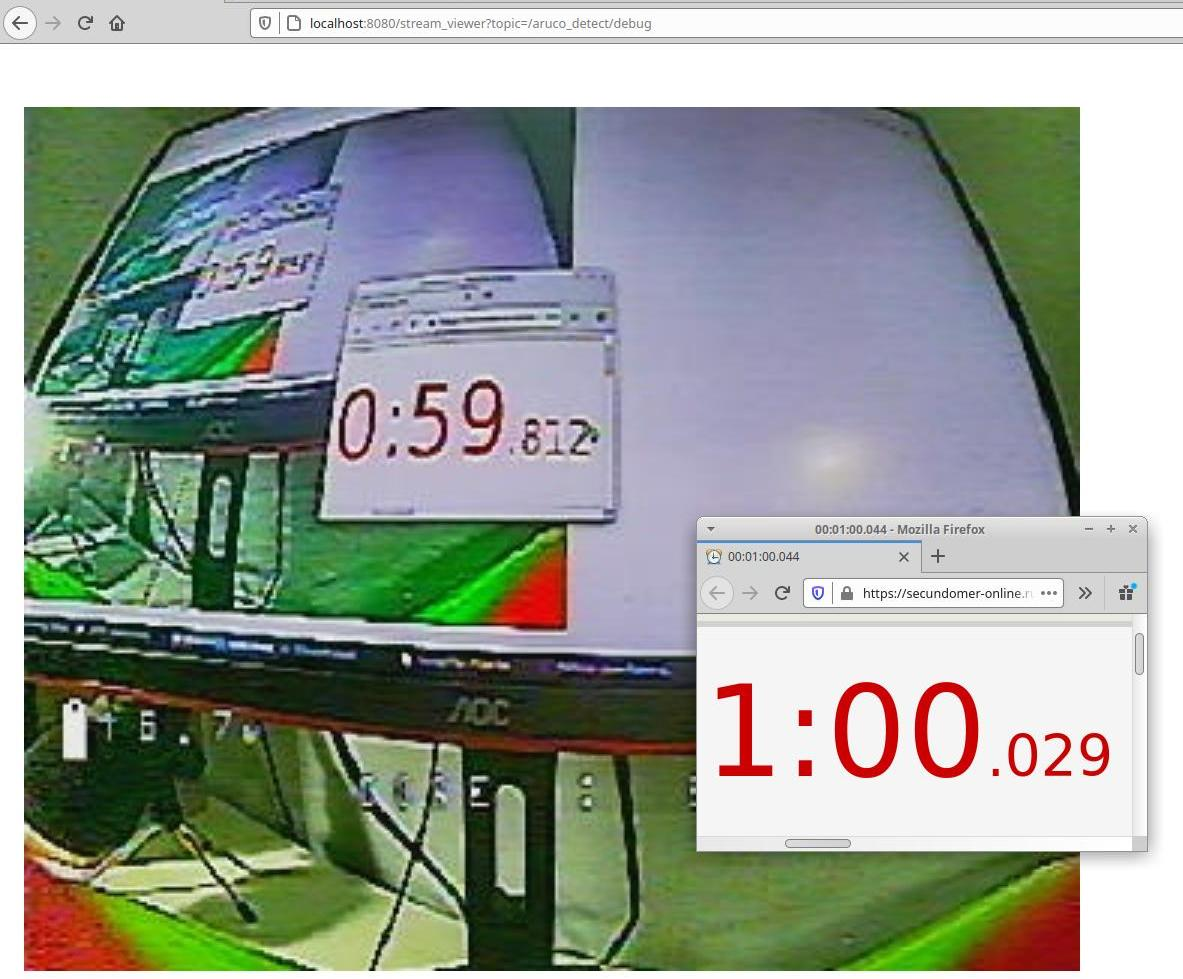
\includegraphics[width=0.5\linewidth]{../RW/pics/time}
	\caption{Задержка аналоговой видеосистемы
	}
	\label{fig:time} % эта метка позволяет ссылаться на рисунок в тексте
\end{figure}

\begin{figure}[H]
	\centering
	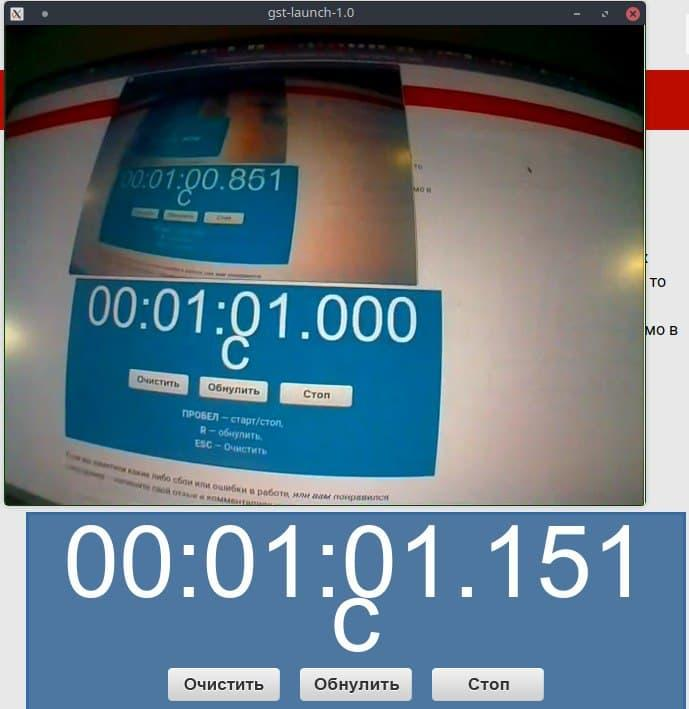
\includegraphics[width=0.5\linewidth]{./pics/time}
	\caption{Задержка цифровой видеосистемы
	}
	\label{fig:zadergka} % эта метка позволяет ссылаться на рисунок в тексте
\end{figure}

На борт квадрокоптера был установлен микрокомпьютер RPi zero w со встроенным wifi-модулем.
Мощность модуля в зависимости от версии RPi составляет 0.03-0.05Вт. При настроенной на нужную частоту антенне и отсутствии препятствий на пути сигнал может распространяться на 1 км.
Стандартным шлейфом к интерфейсу CSI подключается камера размером 60*11.5*5 мм. Угол обзора камеры 72 градуса, разрешение 5 МП. Максимальное разрешение видео составляет 1080p. На рисунке \ref{fig:drone1} представлен собранный образец.

\begin{figure}[H]
	\centering
	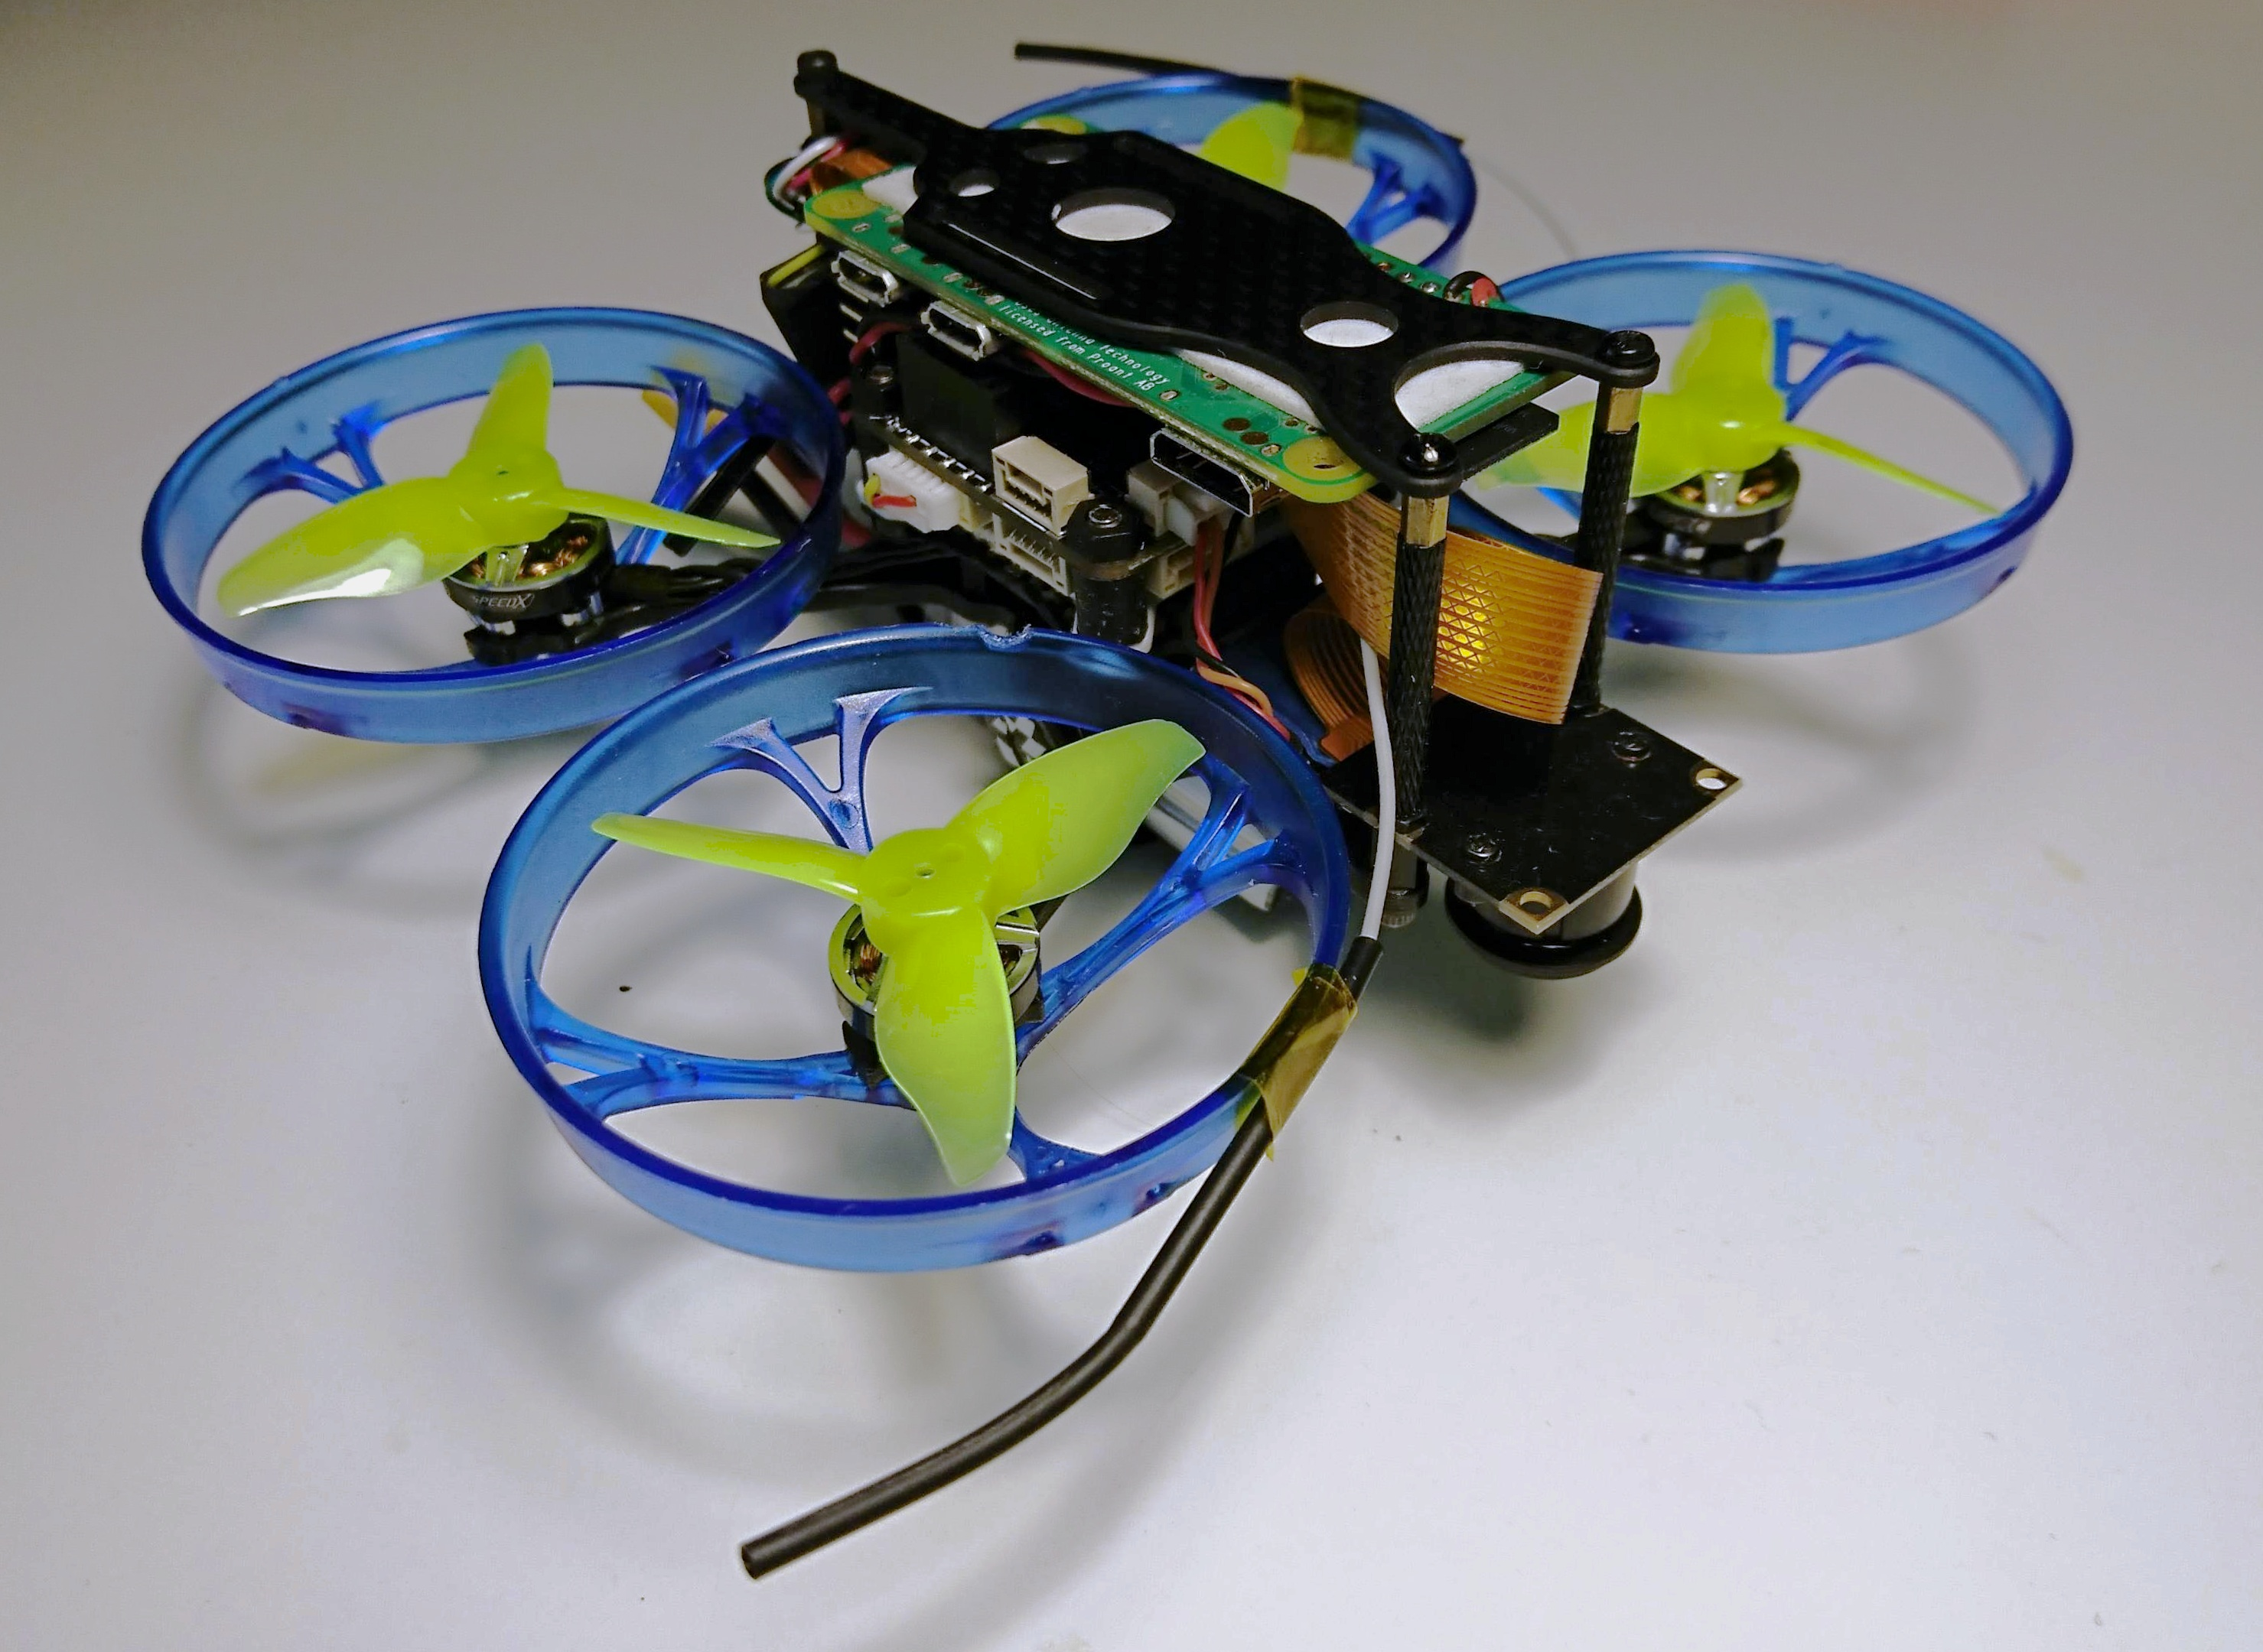
\includegraphics[width=0.5\linewidth]{./pics/drone}
	\caption{Второй экспериментальный образец дрона
	}
	\label{fig:drone1} % эта метка позволяет ссылаться на рисунок в тексте
\end{figure}

После настройки программной части полетного контроллера (прошивки) будет необходима подготовка образа RPi и настройка окружения для трансляции видеопотока с борта дрона.

%\url{https://dev.px4.io/v1.9.0/en/ros/offboard\_control.html}
%\url{https://dev.px4.io/v1.9.0/en/ros/external_position_estimation.html}
\subsection{Настройка дрона для передачи телеметрии и видеопотока на наземную станцию}

\subsubsection{Настройка PX4}
Через конфигуратор qgroundcontrol на полетный контроллер загружается прошивка PX4, после чего необходима первоначальная настройка.

Последовательность действий:
\begin{itemize}
	\item указание прошивке на тип и схему БПЛА (квадрокоптер);
	\item калибровку датчиков (акселерометра, магнитометра, гироскопа...);
	\item проверка корректности ориентации датчиков положения -- акселерометра и гироскопа (отклонения по всем осям происходят в нужные стороны);
	\item конфигурация протокола радиоуправления;
	\item калибровка и настройка каналов радиоуправления (выставлены последовательно соответствующие оси и добавлены необходимые режимы);
	\item проверяется и задается последовательность моторов (порядковые номера моторов соответствуют используемым прошивкой полетного контроллера);
	\item проверяется направление вращений моторов и пропеллеров (диагональные моторы вращаются в одинаковых направлениях согласно выбранной схеме ЛА).
\end{itemize}

Часто в связи с некорректной настройкой одного из описанных пунктов возникают неконтролируемые ситуации при старте -- дрон отказывается взлетать или переворачивается при взлете.

Выставляются полетные режимы:

ACRO -- режим, где отклонением стиков задается угловая скорость для соответствующей оси дрона. Центральное положение стика означает нулевую угловую скорость; в то время как угловая скорость при крайнем положении настраивается значением системы рейтов. Таким образом, при нулевом положении стика дрон не возвращается в горизонт (отсутствует стабилизация уровня). Режим ACRO используется для акробатических полетов, когда требуется плавное и быстрое управление \cite{ardupilot}.

STABILIZED -- режим стабилизации дрона, когда стики аппаратуры находятся в центре; используется для ручного управления в ходе полетных испытаний внутри помещения.

POSHOLD -- удержание позиции по датчикам / компьютерному зрению; когда будет настроена система оценки положения дрона в пространстве, при включении указанного режима дрон должен держаться в одной точке с учетом погрешности.

OFFBOARD -- управление полетом с внешнего компьютера. Этот режим используется для программирования автономных полетов \cite{clover}, при котором управление происходит из выполняемой на внешнем компьютере программы.

После выполнения описанных в начале раздела шагов производится взлет в ручных режимах. Во время полета проверяется ПИД регулирование.

Настройка ПИД-регулятора производится стандартным методом анализа реакции step res\-ponse \cite{step}.

Суть метода заключается в передаче ступенчатого управляющего сигнала на вход регулятора и анализе реакции системы на него.
Медленная реакция на ступенчатый управляющий сигнал указывает на низкий коэффициент пропорциональной составляющей.
Коэффициент увеличивается до появления характерного перерегулирования.
После чего остаточные осцилляции гасятся путем повышения коэффициента дифференциальной составляющей.

Далее изменяются параметры для взаимодействия с Raspberry Pi: указывается используемый порт (UART) и бод-рейт 921600.
По умолчанию MAVLink функционирует в режиме, где передает все имеющиеся сообщения, но для поставленной задачи это не нужно, так как вносится задержка. Первым делом пришла идея сборки для отправки самого необходимого, но оказалось, что от разработчиков уже есть параметр для выбора типа отправляемых сообщений, и был определен тип, где выбраны только сообщения внешнего визуального позиционирования.
Программно отключаются использование компаса и GPS, так как они не устанавливаются на борт дрона, и выставляются параметры для оценки положения по EKF из ECL.

Библиотека оценки и управления (ECL) использует алгоритм расширенного фильтра Калмана (EKF) для обработки измерений датчика и предоставления оценки следующих состояний:
\begin{itemize}
	\item кватернион, определяющий вращение из одной системы отсчета (North, East, Down локальной координатной плоскости) в другую ( X, Y, Z тела);
	\item скорость на IMU -- North, East, Down (м / с);
	\item положение в IMU -- North, East, Down (м);
	\item оценки смещения угла дельты IMU -- X, Y, Z (рад);
	\item оценки смещения дельта-скорости IMU -- X, Y, Z (м / с);
	\item составляющие магнитного поля Земли -- North, East, Down (гаусс);
	\item система координат связанная с телом летательного аппарата -- X, Y, Z (Гаусс);
	\item скорость ветра -- север, восток (м / с).
\end{itemize}

EKF реализует систему <<отложенного временного горизонта слияния>>, что позволяет учесть временные задержки опроса датчиков относительно IMU. Данные для каждого датчика буферизуются FIFO и извлекаются из буфера с помощью EKF для использования в нужное время. Компенсация задержки для каждого датчика регулируется параметрами EKF2*DELAY.

EKF имеет разные режимы работы, которые позволяют использовать различные комбинации опроса датчиков. При запуске фильтр проверяет минимальную жизнеспособную комбинацию датчиков и после завершения начального выравнивания наклона, рыскания и высоты входит в режим, который обеспечивает оценку вращения, вертикальной скорости, вертикального положения, отклонения угла отклонения IMU и отклонения дельта-скорости IMU.

Для этого режима требуются данные IMU, источник рыскания (магнитометр или система внешнего визуального позиционирования (external vision)) и источник данных о высоте. Этот минимальный набор данных требуется для всех режимов работы EKF. Затем данные других датчиков можно использовать для оценки дополнительных состояний \cite{px4}.

В качестве источника картинки для системы внешнего визуального позиционирования используется RPi c камерой. Помимо передачи видеопотока RPi осуществляет приемо-передачу MAVLink сообщений с наземной станции и по UART передает их в полетный контроллер, таким образом убирая необходимость в устройстве приемо-передачи телеметрии.
% дописано
%https://docs.px4.io/master/en/advanced_config/tuning_the_ecl_ekf.html

%https://docs.px4.io/master/en/ros/external_position_estimation.html
%https://docs.px4.io/master/en/peripherals/mavlink_peripherals.html

\subsubsection{Настройка Raspberry Pi}

Для RPi выбрана операционная система raspbian stretch lite -- простая ОС на базе ядра Linux с интерфейсом командной строки (CLI). В ней нет графического интерфейса, и в состав дистрибутива не входит второстепенное / дополнительное программное обеспечение.
%http://www.pcds.fi/downloads/operatingsystem/debianbased/raspbian/archive/stretch/raspbian.stretch.html
С помощью команд, представленных в листинге \ref{lst:5}, был записан образ на карту памяти микрокомпьютера.
\begin{Program}[H]
\caption{Подготовка карты памяти для RPi} \label{lst:5}
\begin{MyCode}
\$ unzip -p 2018-11-13-raspbian-stretch-lite.zip
\$ sudo dd if=/home/qw/2018-11-13-raspbian-stretch-lite.img of=/dev/sdd
\$ sync
\end{MyCode}
\end{Program}

Для подключения к роутеру изменены параметры wpa\_supplicant.conf (листинг \ref{lst:55}).
\begin{Program}[H]
\caption{Настройка подключения RPi к роутеру} \label{lst:55}
\begin{MyCode}
$ less /etc/wpa_supplicant/wpa_supplicant.conf
ctrl_interface=DIR=/var/run/wpa_supplicant GROUP=netdev
update_config=1
country=RU

network={
	ssid=<<ИМЯ_ТОЧКИ_ДОСТУПА>>
	psk=passwd
}
	\end{MyCode}
\end{Program}

Для того, чтобы на RPi активировать возможность удаленного подключения по протоколу ssh, необходимо запустить сервис ssh. Это возможно путем создания пустого файла с названием ssh в каталоге /boot. 
% дописано
%https://habr.com/ru/post/419947/

После выполнения описанных шагов microSD карта вставляется в RPi. Для удаленного подключения необходимо просканировать сеть и найти ip-адрес RPi. Это возможно с помощью утилиты nmap на наземной станции (листинг \ref{lst:6}).
\begin{Program}[H]
	\caption{Поиск адресов в подсети роутера} \label{lst:6}
\begin{MyCode}
$ sudo nmap -sn 192.168.1.0/24
...
Nmap scan report for 192.168.1.148
Host is up (-0.062s latency).
MAC Address: B8:27:EB:D3:B7:09 (Raspberry Pi Foundation)
Nmap scan report for ikherty (192.168.1.28)
Host is up.
Nmap done: 256 IP addresses (4 hosts up) scanned in 4.42 seconds
...
\end{MyCode}
\end{Program}

192.168.1.148 -- ip-адрес Raspberry Pi, назначенный используемым роутером.

%https://www.raspberrypi.org/documentation/remote-access/ip-address.md
Производится удаленное подключение по ssh по найденному адресу, и устанавливаются пакеты gstreamer для запуска трансляции видео с борта дрона.
Для обмена данными между полетным контроллером и RPi устанавливается пакет ser2net и в конфигурационном файле /etc/ser2net.conf добавляется строка, определяющая способ общения, в данном случае она выглядит так (листинг \ref{lst:7}):
\begin{Program}[H]
\caption{Параметры для обмена сообщениями между полетным контроллером и RPi} \label{lst:7}
	\begin{MyCode}
	2000:raw:0:/dev/ttyAMA0:115200 8DATABITS NONE 1STOPBIT
	\end{MyCode}
\end{Program}

%дописать как работает и формат строки сер2нет
В случае с Raspberry источником видеопотока (element1) является rpi\-cam\-src, который захватывает изображение с RPi камеры. rpi\-cam\-src может выводить видео в виде необработанных кадров или закодированное в формате (M)JPEG или H.264 \cite{gstreamer1}. В качестве element2 будет выступать устройство вывода udpsink,-- это сетевой приемник, который отправляет UDP-пакеты в сеть.

Для использования RPi камеры в качестве источника данных трансляции производится сборка gst-rpicamsrc из репозитория \url{https://github.com/thaytan/gst-rpicamsrc} с помощью команд, представленных в листинге \ref{lst:8}:
\begin{Program}[H]
\caption{Сборка rpicamsrc} \label{lst:8}
\begin{MyCode}
$ git clone https://github.com/thaytan/gst-rpicamsrc
$ cd gst-rpicamsrc
$ make
$ make install
\end{MyCode}
\end{Program}


Все необходимые изменения внесены, далее следует произвести настройку наземной станции.

 % вторая глава - в файле part2.tex
\pagebreak
\section{Разработка архитектуры наземной станции}
Аппаратная часть наземной станции изначально состояла из:
\begin{itemize}
	\item компьютера;
	\item передающего модуля радиоуправления;
	\item видеоприемника;
	\item устройства приема-передачи телеметрии.
\end{itemize}

Планировалось, что наземная станция должна обмениваться телеметрией с квадрокоптером, получать видеопоток с квадрокоптера, и отправлять управляющий сигнал в виде команд MAVROS. Чем больше бод -- рейт подключенных модулей и меньше задержка сигнала, тем быстрее осуществляется выполнение команд. Для устройств приема-передачи телеметрии рекомендуется бод -- рейт, равный 921600. Учитывая эти факторы, выбираются устройства телеметрии и видеоприемник.
К компьютеру по UART порту подключается модуль радиоуправления и устройство приема-передачи телеметрии. Через USB порт подключается видеоприемник. Настраивается видеоприемник на диапазон частот, соответствующий частотам видеопередатчика квадрокоптера и далее следует настройка программной части.

Однако в ходе выполнения научно-исследовательской работы \cite{nir3} был выявлен более оптимальный способ обмена информации -- по wifi-соединению. Оно позволяет как уменьшить задержку, количество компонентов, а значит и стоимость комплекта, так и использовать персональный компьютер в качестве наземной станции, куда необходимо поставить несколько программных решений и настроить взаимодействие между ними.

Программная часть представляет собой совокупность взаимодействущего программного обеспечения, включающего в себя:
\begin{itemize}
	\item операционную систему на базе ядра linux;
	\item пакет clover;
	\item qgroundcontrol.
\end{itemize}

qgroundcontrol необходим для настройки прошивки дрона и отслеживания предупреждений в случае неисправностей.
По MAVLink протоколу передаются данные в указанный UART, и все программы, прослушивающие этот UART, порт имеют доступ к данным с борта квадрокоптера. Для взаимодействия через ROS инструменты необходима настройка всех параметров подключения. На данном этапе НИР используется готовой решение от Copter Express -- пакет clover, позволяющий производить настройку максимально просто. В launch файлах пакета прописываются все параметры. Указывается UART, бауд -- рейт, и в консоли запускается clover с помощью команд, представленных в листинге \ref{lst:45}:
\begin{Program}[H]
	\caption{Запуск clover} \label{lst:45}
	\begin{MyCode}
	gs@groundstation:~$ source /home/clover/catkin\_ws/devel/setup.bash
	gs@groundstation:~$ roslaunch clover clover.launch
	\end{MyCode}
\end{Program}

После этого доступны все инструменты clover. На листинге \ref{lst:5} приведен результат выполнения команды для получения телеметрии. "frame\_id: ''" означает, что показания берутся в системе координат относительно квадрокоптера.
\begin{Program}[H]
	\caption{Вывод телеметрии квадрокоптера в консоли} \label{lst:5}
	\begin{MyCode}
	gs@groundstation:~$ rosservice call /get_telemetry "frame_id: ''" 
	frame_id: "map"
	connected: True
	armed: False
	mode: "MANUAL"
	x: -0.00260298536159
	y: -6.72723326716e-05
	z: 0.00103790743742
	lat: 0.0
	lon: 0.0
	alt: 0.0
	vx: -0.00717502878979
	vy: -0.00176917202771
	vz: 0.00364218326285
	pitch: 0.0221049506217
	roll: -0.0172985047102
	yaw: 0.000302107335301
	pitch_rate: 0.00245076417923
	roll_rate: 0.00449034944177
	yaw_rate: 0.00266480189748
	voltage: 12.1499996185
	cell_voltage: 4.05000019073
	gs@groundstation:~$
	\end{MyCode}
\end{Program}

Видеоприемник подключен в порт /dev/video0. Он указывается в launch-файле, далее перезагружается clover и проверяются в web-браузере топики по адресу localhost:8080 (рисунок \ref{fig:topic}).

\begin{figure}[H]
	\centering
	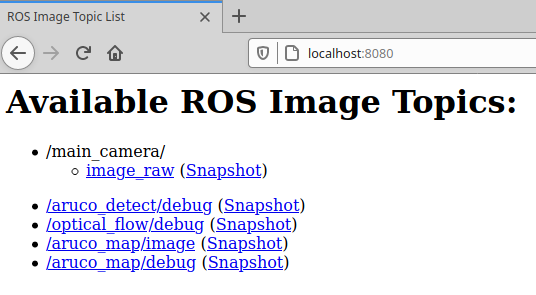
\includegraphics[width=0.5\linewidth]{../RW/pics/topic}
	\caption{Список топиков, доступный по умолчанию
	}
	\label{fig:topic}
\end{figure}

Список НОД также меняется в launch файлах. В image raw топике будет отображаться видеопоток, полученный видеоприемником с борта квадрокоптера, в остальных топиках публикуются:
\begin{itemize}
	\item aruco-detect (на image raw определяются с помощью openCV aruco маркеры);
	\item optical flow (на изображение с image raw накладывается точка отсчета для лазерного дальномера);
	\item aruco map (карта маркеров, прописанная в конфигурационном файле).
\end{itemize}

Optical flow отключается, так как на БПЛА не установлен лазерный дальномер.
\subsection{Конфигурация наземной станции}
Наземная станция представляет собой компьютер, подключенный к тому же роутеру, что и дрон. Операционная система на базе ядра linux, установлены пакеты ros, соответствующие версии ОС, в данном случае ros-melodic-full, и gstreamer для приема видеопотока.

\subsection{Настройка mavros}
Для того, чтобы ноды могли обмениваться данными, необходим roscore \cite{pkg}. roscore - это набор нод и программ, которые являются предпосылками системы на основе ROS \cite{ros}. Запускается с помощью команды \$ roscore в одной из вкладок консоли, однако при использовании roslaunch это действие необязательно -- при выполнении roslaunch первым делом запускается roscore.

roslaunch - это инструмент для простого запуска нескольких нод ROS. Он включает в себя опции для автоматического запуска уже завершенных процессов. roslaunch принимает один или несколько файлов конфигурации XML (с расширением .launch), определяющих параметры, которые необходимо установить, и ноды для запуска, а также машины, на которых они должны запускаться \cite{ros}.

Для получения телеметрии полетного контроллера в /opt/ros/melodic/sha\-re/mavros/launch/px4.launch файле поменять параметры fcu\_url, указав нужный адрес и порт. Видеопоток планируется получать UDP пакетами, для их обработки необходимо указать адрес и порт в параметре gcs\_url (листинг \ref{lst:9}):
\begin{Program}[H]
	\caption{Измененные параметры в launch файле mavros} \label{lst:9}
	\begin{MyCode}
	<arg name="fcu_url" default="tcp://192.168.1.148:2000?ids=1,240"/>   
	<arg name="gcs_url" default="udp://@127.0.0.1:14555"/>
	\end{MyCode}
\end{Program}

\subsection{Подготовка инструментов для получения и обработки видеопотока}
Для получения трансляции и публикации топиков с изображением с камеры используется gscam. Он собирается из репозитория \url{https://github.com/ros-drivers/gscam} командами, представленными в листинге \ref{lst:10}:
\begin{Program}[H]
	\caption{Сборка gscam} \label{lst:10}
	\begin{MyCode}
	$ git clone https://github.com/ros-drivers/gscam
	$ cd gscam
	$ cmake -DGSTREAMER_VERSION_1_x=On
	$ сmake install
	\end{MyCode}
\end{Program}

Распознавание карты aruco маркеров на изображении, получаемом из топиков gscam, и публикацию полученных координат в топик /vision/pose производит aruco\_gridboard. Команды для сборки этого пакета представлены в листинге \ref{lst:11}:
\begin{Program}[H]
	\caption{Сборка aruco\_gridboard} \label{lst:11}
	\begin{MyCode}	
	$ cd ~/catkin_ws/src
	$ git clone https://github.com/anbello/aruco_gridboard.git
	$ cd ..
	$ catkin_make
	$ source devel/setup.bash
	$ catkin_make --only-pkg-with-deps aruco_gridboard
	\end{MyCode}
\end{Program}

Проделанных шагов достаточно, чтобы на наземной станции отобразить положение дрона относительно карты маркеров.
  % третья глава - в файле part3.tex
\pagebreak

\section{Протоколы общения дрона и наземной станции}
\subsection{Структура пакета}
Рассмотрим подробнее устройство MAVLink. Ниже приведена структура пакета MAVLink v2. Представление в памяти может отличаться.

uint8\_t magic;              //Метка начала

uint8\_t len;                //Размер данных/длинна полезной нагрузки (сообщения)

uint8\_t incompat\_flags;     //Обратно несовместимые флаги

uint8\_t compat\_flags;       //Обратно совместимые флаги

uint8\_t seq;                //Порядковый номер сообщения для выявления потери сообщения

uint8\_t sysid;              //ID системы-отправителя

uint8\_t compid;             //ID компонента-отправителя

uint8\_t msgid 0:7;          //ID сообщения (первый байт), от него зависит, какие данные будут лежать в полезной нагрузке пакета

uint8\_t msgid 8:15;         //ID сообщения (второй байт)

uint8\_t msgid 16:23;        //ID сообщения (третий байт)

uint8\_t payload[max 255];   //Полезная нагрузка (размер сообщения максимум 255 байт) 

uint16\_t checksum;          //Контрольная сумма

uint8\_t signature[13];      //Сигнатура (опционально)

Структура пакета MAVLink v1 аналогична, но опускает incompat\_flags, compat\_flags и signature, и имеет только один байт для адреса сообщения.


\subsection{Публикация}
Беспроводной формат MAVLink оптимизирован для систем с ограниченными ресурсами и, следовательно, порядок полей не такой, как в спецификации XML. Беспроводной генератор сортирует все поля сообщения по размеру, сначала с самыми большими полями (uint64\_t), а затем с меньшими полями. Сортировка выполняется с использованием стабильного алгоритма сортировки, который гарантирует, что любые поля, которые не нужно переупорядочивать, останутся в том же относительном порядке. Это предотвращает проблемы с выравниванием в системах кодирования / декодирования и позволяет очень эффективно упаковывать / распаковывать.

\subsection{Многоадресные потоки и гарантированная доставка}
MAVLink создан для гибридных сетей, в которых высокоскоростные потоки данных от источников данных (беспилотных летательных аппаратов) поступают в приемники данных (наземные станции), но смешиваются с передачами, требующими гарантированной доставки. Ключевой вывод состоит в том, что для большинства потоков телеметрии не существует известного или единственного получателя: вместо этого, как правило, бортовой компьютер, наземная станция управления и облачная система нуждаются в одном и том же потоке данных.

С другой стороны, настройка бортовой миссии или изменение конфигурации системы с бортовыми параметрами требует точка-точка связи с гарантированной доставкой. MAVLink достигает очень высокой эффективности за счет использования обоих режимов работы.

\subsection{Режим топиков (публикация-подписка)}
%написать про топики и подписки
В режиме топиков протокол не будет выдавать идентификатор целевой системы и компонента для сообщений, чтобы сэкономить пропускную способность канала. Типичными примерами этого режима связи являются все потоки данных автопилота, такие как положение, координаты и т. д.

Основное преимущество этого режима заключается в том, что не создаются дополнительные накладные расходы, и все подписчики могут получать эти данные.

\subsection{Соединение точка-точка}% топология?

В режиме точка-точка MAV\-Link использует идентификатор цели и целевой компонент. В большинстве случаев, когда используются эти поля, подпротокол также обеспечивает гарантированную доставку (миссии, параметры, команды).

\subsection{Проверки целостности}
MAV\-Link реализует две проверки целостности: первая проверка целостности пакета во время передачи с использованием контрольной суммы X.25 ( $CRC-16-CCITT$ ). Однако это только гарантирует, что данные не были изменены в ссылке -- это не гарантирует согласованности с определением данных. Вторая проверка целостности связана с описанием данных, чтобы убедиться в содержании идентичной информации у двух сообщений с одинаковым идентификатором. Для этого само определение данных проходит через $CRC-16-CCITT$, а полученное значение используется для заполнения пакета CRC. Большинство эталонных реализаций хранят эту константу в массиве CRC\_EXTRA \cite{mavlink}.

% из хабра

Библиотека MAV\-Link позволяет кодировать и раскодировать пакеты согласно протоколу, но она не регламентирует, какими аппаратными и программными средствами данные будет отправлены — это могут быть TCP/UDP сообщения, обмен через последовательный порт, - все, что обеспечивает двухсторонний обмен. Библиотека обрабатывает входные данные побайтово, добавляя их в буфер и сама собирает из них пакет. Каждая система или компонент, может одновременно обмениваться данными по разным источникам, тогда для каждого источника назначается специальный идентификатор, называемый channel (канал). MAV\-Link содержит буфер на каждый канал.

%\url{https://habr.com/ru/post/312300/}

Канал связи
Протокол MAV\-Link может быть использован поверх следующих каналов связи:
последовательное соединение (UART, USB и др.);
UDP (Wi-Fi, Ethernet, 3G, LTE);
TCP (Wi-Fi, Ethernet, 3G, LTE).
Сообщение
MAV\-Link-сообщение это отдельная "порция" данных, передаваемая между устройствами. Отдельное MAV\-Link-сообщение содержит информацию о состоянии дрона или команду для дрона.

Примеры MAV\-Link-сообщений:
ATTITUDE, ATTITUDE\_QUATERNION – ориентация квадрокоптера в пространстве;
LOCAL\_POSITION\_NED – локальная позиция квадрокоптера;
GLOBAL\_POSITION\_INT – глобальная позиция квадрокоптера (широта/долгота/высота);
COMMAND\_LONG – команда для квадрокоптера (взлететь, сесть, переключить режим и т. д.).

%\url{https://clover.coex.tech/ru/mavlink.html}


%//осознанно переписать

%//подвести итог, чем полезно, как улучшить для наших целей(возможно, одна из задач на следующий семестр) 

 % четвертая глава - в файле part4.tex
\pagebreak

\section*{\centering ЗАКЛЮЧЕНИЕ}
\addcontentsline{toc}{section}{ЗАКЛЮЧЕНИЕ}

В ходе проделанной работы была проведена --- описать результаты бурной деятельности по выполнению ВКР, разумно в виде списка выполненных задач.

Разработанная программа позволяет --- перечислить основные функциональные характеристики и особенности, можно в виде списка:
\begin{itemize}
\item выполнено такое-то задание;
\item разработана некоторая система;
\item у работы есть перспективы развития.
\end{itemize}

% оформление библиографии - вариант с БД
\pagebreak

\addcontentsline{toc}{section}{СПИСОК ИСПОЛЬЗОВАННЫХ ИСТОЧНИКОВ}
% ВАЖНО: для корректного отображения в списке литературы ссылок на англ.языке в bibtex-описание источника следует добавить поле 
% langid = {english}
\printbibliography

\pagebreak

\end{document}          

